\documentclass[twoside]{book}

% Packages required by doxygen
\usepackage{fixltx2e}
\usepackage{calc}
\usepackage{doxygen}
\usepackage[export]{adjustbox} % also loads graphicx
\usepackage{graphicx}
\usepackage[utf8]{inputenc}
\usepackage{makeidx}
\usepackage{multicol}
\usepackage{multirow}
\PassOptionsToPackage{warn}{textcomp}
\usepackage{textcomp}
\usepackage[nointegrals]{wasysym}
\usepackage[table]{xcolor}

% Font selection
\usepackage[T1]{fontenc}
\usepackage[scaled=.90]{helvet}
\usepackage{courier}
\usepackage{amssymb}
\usepackage{sectsty}
\renewcommand{\familydefault}{\sfdefault}
\allsectionsfont{%
  \fontseries{bc}\selectfont%
  \color{darkgray}%
}
\renewcommand{\DoxyLabelFont}{%
  \fontseries{bc}\selectfont%
  \color{darkgray}%
}
\newcommand{\+}{\discretionary{\mbox{\scriptsize$\hookleftarrow$}}{}{}}

% Page & text layout
\usepackage{geometry}
\geometry{%
  a4paper,%
  top=2.5cm,%
  bottom=2.5cm,%
  left=2.5cm,%
  right=2.5cm%
}
\tolerance=750
\hfuzz=15pt
\hbadness=750
\setlength{\emergencystretch}{15pt}
\setlength{\parindent}{0cm}
\setlength{\parskip}{0.2cm}
\makeatletter
\renewcommand{\paragraph}{%
  \@startsection{paragraph}{4}{0ex}{-1.0ex}{1.0ex}{%
    \normalfont\normalsize\bfseries\SS@parafont%
  }%
}
\renewcommand{\subparagraph}{%
  \@startsection{subparagraph}{5}{0ex}{-1.0ex}{1.0ex}{%
    \normalfont\normalsize\bfseries\SS@subparafont%
  }%
}
\makeatother

% Headers & footers
\usepackage{fancyhdr}
\pagestyle{fancyplain}
\fancyhead[LE]{\fancyplain{}{\bfseries\thepage}}
\fancyhead[CE]{\fancyplain{}{}}
\fancyhead[RE]{\fancyplain{}{\bfseries\leftmark}}
\fancyhead[LO]{\fancyplain{}{\bfseries\rightmark}}
\fancyhead[CO]{\fancyplain{}{}}
\fancyhead[RO]{\fancyplain{}{\bfseries\thepage}}
\fancyfoot[LE]{\fancyplain{}{}}
\fancyfoot[CE]{\fancyplain{}{}}
\fancyfoot[RE]{\fancyplain{}{\bfseries\scriptsize Generated on Wed Apr 1 2015 23\+:15\+:37 for multi\+Touch\+Sample by Doxygen }}
\fancyfoot[LO]{\fancyplain{}{\bfseries\scriptsize Generated on Wed Apr 1 2015 23\+:15\+:37 for multi\+Touch\+Sample by Doxygen }}
\fancyfoot[CO]{\fancyplain{}{}}
\fancyfoot[RO]{\fancyplain{}{}}
\renewcommand{\footrulewidth}{0.4pt}
\renewcommand{\chaptermark}[1]{%
  \markboth{#1}{}%
}
\renewcommand{\sectionmark}[1]{%
  \markright{\thesection\ #1}%
}

% Indices & bibliography
\usepackage{natbib}
\usepackage[titles]{tocloft}
\setcounter{tocdepth}{3}
\setcounter{secnumdepth}{5}
\makeindex

% Hyperlinks (required, but should be loaded last)
\usepackage{ifpdf}
\ifpdf
  \usepackage[pdftex,pagebackref=true]{hyperref}
\else
  \usepackage[ps2pdf,pagebackref=true]{hyperref}
\fi
\hypersetup{%
  colorlinks=true,%
  linkcolor=blue,%
  citecolor=blue,%
  unicode%
}

% Custom commands
\newcommand{\clearemptydoublepage}{%
  \newpage{\pagestyle{empty}\cleardoublepage}%
}


%===== C O N T E N T S =====

\begin{document}

% Titlepage & ToC
\hypersetup{pageanchor=false,
             bookmarks=true,
             bookmarksnumbered=true,
             pdfencoding=unicode
            }
\pagenumbering{roman}
\begin{titlepage}
\vspace*{7cm}
\begin{center}%
{\Large multi\+Touch\+Sample \\[1ex]\large 1.\+0.\+0 }\\
\vspace*{1cm}
{\large Generated by Doxygen 1.8.9.1}\\
\vspace*{0.5cm}
{\small Wed Apr 1 2015 23:15:37}\\
\end{center}
\end{titlepage}
\clearemptydoublepage
\tableofcontents
\clearemptydoublepage
\pagenumbering{arabic}
\hypersetup{pageanchor=true}

%--- Begin generated contents ---
\chapter{Namespace Index}
\section{Packages}
Here are the packages with brief descriptions (if available)\+:\begin{DoxyCompactList}
\item\contentsline{section}{\hyperlink{namespacecom}{com} }{\pageref{namespacecom}}{}
\item\contentsline{section}{\hyperlink{namespacecom_1_1example}{com.\+example} }{\pageref{namespacecom_1_1example}}{}
\item\contentsline{section}{\hyperlink{namespacecom_1_1example_1_1multitouchsample}{com.\+example.\+multitouchsample} }{\pageref{namespacecom_1_1example_1_1multitouchsample}}{}
\end{DoxyCompactList}

\chapter{Hierarchical Index}
\section{Class Hierarchy}
This inheritance list is sorted roughly, but not completely, alphabetically\+:\begin{DoxyCompactList}
\item \contentsline{section}{com.\+example.\+multitouchsample.\+Main\+Activity.\+My\+View.\+Circle\+Linked\+With\+Pt\+Id}{\pageref{classcom_1_1example_1_1multitouchsample_1_1_main_activity_1_1_my_view_1_1_circle_linked_with_pt_id}}{}
\item \contentsline{section}{com.\+example.\+multitouchsample.\+Main\+Activity.\+My\+View.\+Pt\+Id\+Linked\+With\+Pt\+Index}{\pageref{classcom_1_1example_1_1multitouchsample_1_1_main_activity_1_1_my_view_1_1_pt_id_linked_with_pt_index}}{}
\item Activity\begin{DoxyCompactList}
\item \contentsline{section}{com.\+example.\+multitouchsample.\+Main\+Activity}{\pageref{classcom_1_1example_1_1multitouchsample_1_1_main_activity}}{}
\end{DoxyCompactList}
\item View\begin{DoxyCompactList}
\item \contentsline{section}{com.\+example.\+multitouchsample.\+Main\+Activity.\+My\+View}{\pageref{classcom_1_1example_1_1multitouchsample_1_1_main_activity_1_1_my_view}}{}
\end{DoxyCompactList}
\end{DoxyCompactList}

\chapter{Class Index}
\section{Class List}
Here are the classes, structs, unions and interfaces with brief descriptions\+:\begin{DoxyCompactList}
\item\contentsline{section}{\hyperlink{classcom_1_1example_1_1multitouchsample_1_1_main_activity_1_1_my_view_1_1_circle_linked_with_pt_id}{com.\+example.\+multitouchsample.\+Main\+Activity.\+My\+View.\+Circle\+Linked\+With\+Pt\+Id} }{\pageref{classcom_1_1example_1_1multitouchsample_1_1_main_activity_1_1_my_view_1_1_circle_linked_with_pt_id}}{}
\item\contentsline{section}{\hyperlink{classcom_1_1example_1_1multitouchsample_1_1_main_activity}{com.\+example.\+multitouchsample.\+Main\+Activity} }{\pageref{classcom_1_1example_1_1multitouchsample_1_1_main_activity}}{}
\item\contentsline{section}{\hyperlink{classcom_1_1example_1_1multitouchsample_1_1_main_activity_1_1_my_view}{com.\+example.\+multitouchsample.\+Main\+Activity.\+My\+View} }{\pageref{classcom_1_1example_1_1multitouchsample_1_1_main_activity_1_1_my_view}}{}
\item\contentsline{section}{\hyperlink{classcom_1_1example_1_1multitouchsample_1_1_main_activity_1_1_my_view_1_1_pt_id_linked_with_pt_index}{com.\+example.\+multitouchsample.\+Main\+Activity.\+My\+View.\+Pt\+Id\+Linked\+With\+Pt\+Index} }{\pageref{classcom_1_1example_1_1multitouchsample_1_1_main_activity_1_1_my_view_1_1_pt_id_linked_with_pt_index}}{}
\end{DoxyCompactList}

\chapter{File Index}
\section{File List}
Here is a list of all files with brief descriptions\+:\begin{DoxyCompactList}
\item\contentsline{section}{src/com/fouram/nurumikeyboard/\+Nurumi\+I\+M\+E/\hyperlink{_m_keyboard_view_8java}{M\+Keyboard\+View.\+java} }{\pageref{_m_keyboard_view_8java}}{}
\item\contentsline{section}{src/com/fouram/nurumikeyboard/\+Nurumi\+I\+M\+E/\hyperlink{_nurumi_i_m_e_8java}{Nurumi\+I\+M\+E.\+java} }{\pageref{_nurumi_i_m_e_8java}}{}
\item\contentsline{section}{src/com/fouram/nurumikeyboard/\+Nurumi\+I\+M\+E/\hyperlink{_on_m_keyboard_gesture_listener_8java}{On\+M\+Keyboard\+Gesture\+Listener.\+java} }{\pageref{_on_m_keyboard_gesture_listener_8java}}{}
\end{DoxyCompactList}

\chapter{Namespace Documentation}
\hypertarget{namespacecom}{}\section{Package com}
\label{namespacecom}\index{com@{com}}
\subsection*{Packages}
\begin{DoxyCompactItemize}
\item 
package \hyperlink{namespacecom_1_1example}{example}
\end{DoxyCompactItemize}

\hypertarget{namespacecom_1_1example}{}\section{Package com.\+example}
\label{namespacecom_1_1example}\index{com.\+example@{com.\+example}}
\subsection*{Packages}
\begin{DoxyCompactItemize}
\item 
package \hyperlink{namespacecom_1_1example_1_1multitouchsample}{multitouchsample}
\end{DoxyCompactItemize}

\hypertarget{namespacecom_1_1example_1_1multitouchsample}{}\section{Package com.\+example.\+multitouchsample}
\label{namespacecom_1_1example_1_1multitouchsample}\index{com.\+example.\+multitouchsample@{com.\+example.\+multitouchsample}}
\subsection*{Classes}
\begin{DoxyCompactItemize}
\item 
class \hyperlink{classcom_1_1example_1_1multitouchsample_1_1_main_activity}{Main\+Activity}
\end{DoxyCompactItemize}

\chapter{Class Documentation}
\hypertarget{classcom_1_1example_1_1multitouchsample_1_1_main_activity_1_1_my_view_1_1_circle_linked_with_pt_id}{}\section{com.\+example.\+multitouchsample.\+Main\+Activity.\+My\+View.\+Circle\+Linked\+With\+Pt\+Id Class Reference}
\label{classcom_1_1example_1_1multitouchsample_1_1_main_activity_1_1_my_view_1_1_circle_linked_with_pt_id}\index{com.\+example.\+multitouchsample.\+Main\+Activity.\+My\+View.\+Circle\+Linked\+With\+Pt\+Id@{com.\+example.\+multitouchsample.\+Main\+Activity.\+My\+View.\+Circle\+Linked\+With\+Pt\+Id}}


Collaboration diagram for com.\+example.\+multitouchsample.\+Main\+Activity.\+My\+View.\+Circle\+Linked\+With\+Pt\+Id\+:
\nopagebreak
\begin{figure}[H]
\begin{center}
\leavevmode
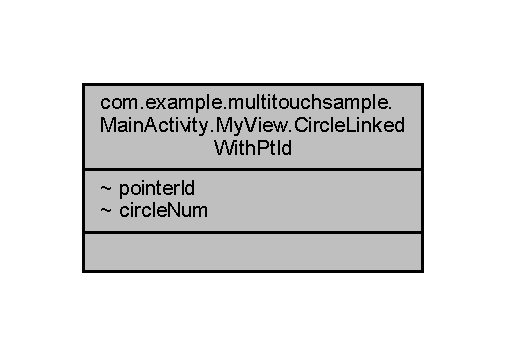
\includegraphics[width=243pt]{classcom_1_1example_1_1multitouchsample_1_1_main_activity_1_1_my_view_1_1_circle_linked_with_pt_id__coll__graph}
\end{center}
\end{figure}


\subsection{Detailed Description}
\hyperlink{namespacecom_1_1example_1_1multitouchsample}{com.\+example.\+multitouchsample} ~\newline
 �� \hyperlink{_main_activity_8java}{Main\+Activity.\+java} \hypertarget{classcom_1_1example_1_1multitouchsample_1_1_main_activity_1_1_my_view_1_1_pt_id_linked_with_pt_index_Class}{}\subsection{information}\label{classcom_1_1example_1_1multitouchsample_1_1_main_activity_1_1_my_view_1_1_pt_id_linked_with_pt_index_Class}
\begin{TabularC}{2}
\hline
\rowcolor{lightgray}\PBS\centering {\bf Item }&{\bf Contents  }\\\cline{1-2}
\PBS\centering Company &4\+:00 A.\+M. \\\cline{1-2}
\PBS\centering Author &Park, Hyung Soon \\\cline{1-2}
\PBS\centering Date &2015. 3. 26. \\\cline{1-2}
\end{TabularC}
\hypertarget{classcom_1_1example_1_1multitouchsample_1_1_main_activity_1_1_my_view_1_1_pt_id_linked_with_pt_index_Description}{}\subsection{Description}\label{classcom_1_1example_1_1multitouchsample_1_1_main_activity_1_1_my_view_1_1_pt_id_linked_with_pt_index_Description}

\begin{DoxyItemize}
\item This class will bind pointer\+I\+D with circle\+Num 
\end{DoxyItemize}

Definition at line 61 of file Main\+Activity.\+java.



The documentation for this class was generated from the following file\+:\begin{DoxyCompactItemize}
\item 
src/com/example/multitouchsample/\hyperlink{_main_activity_8java}{Main\+Activity.\+java}\end{DoxyCompactItemize}

\hypertarget{classcom_1_1example_1_1multitouchsample_1_1_main_activity}{}\section{com.\+example.\+multitouchsample.\+Main\+Activity Class Reference}
\label{classcom_1_1example_1_1multitouchsample_1_1_main_activity}\index{com.\+example.\+multitouchsample.\+Main\+Activity@{com.\+example.\+multitouchsample.\+Main\+Activity}}


Inheritance diagram for com.\+example.\+multitouchsample.\+Main\+Activity\+:
\nopagebreak
\begin{figure}[H]
\begin{center}
\leavevmode
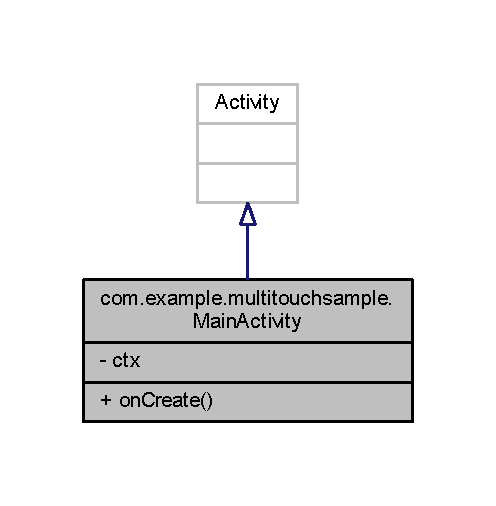
\includegraphics[width=238pt]{classcom_1_1example_1_1multitouchsample_1_1_main_activity__inherit__graph}
\end{center}
\end{figure}


Collaboration diagram for com.\+example.\+multitouchsample.\+Main\+Activity\+:
\nopagebreak
\begin{figure}[H]
\begin{center}
\leavevmode
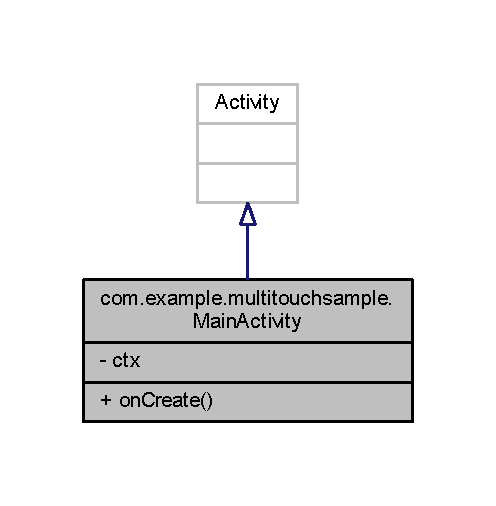
\includegraphics[width=238pt]{classcom_1_1example_1_1multitouchsample_1_1_main_activity__coll__graph}
\end{center}
\end{figure}
\subsection*{Classes}
\begin{DoxyCompactItemize}
\item 
class \hyperlink{classcom_1_1example_1_1multitouchsample_1_1_main_activity_1_1_my_view}{My\+View}
\end{DoxyCompactItemize}
\subsection*{Public Member Functions}
\begin{DoxyCompactItemize}
\item 
void \hyperlink{classcom_1_1example_1_1multitouchsample_1_1_main_activity_a1df850351e22c50dc668c76d8172dc9f}{on\+Create} (Bundle saved\+Instance\+State)
\end{DoxyCompactItemize}
\subsection*{Private Attributes}
\begin{DoxyCompactItemize}
\item 
Context \hyperlink{classcom_1_1example_1_1multitouchsample_1_1_main_activity_a55ac0e8368b828f2e73446810af25a24}{ctx} = this
\end{DoxyCompactItemize}


\subsection{Detailed Description}


Definition at line 18 of file Main\+Activity.\+java.



\subsection{Member Function Documentation}
\hypertarget{classcom_1_1example_1_1multitouchsample_1_1_main_activity_a1df850351e22c50dc668c76d8172dc9f}{}\index{com\+::example\+::multitouchsample\+::\+Main\+Activity@{com\+::example\+::multitouchsample\+::\+Main\+Activity}!on\+Create@{on\+Create}}
\index{on\+Create@{on\+Create}!com\+::example\+::multitouchsample\+::\+Main\+Activity@{com\+::example\+::multitouchsample\+::\+Main\+Activity}}
\subsubsection[{on\+Create}]{\setlength{\rightskip}{0pt plus 5cm}void com.\+example.\+multitouchsample.\+Main\+Activity.\+on\+Create (
\begin{DoxyParamCaption}
\item[{Bundle}]{saved\+Instance\+State}
\end{DoxyParamCaption}
)}\label{classcom_1_1example_1_1multitouchsample_1_1_main_activity_a1df850351e22c50dc668c76d8172dc9f}
Called when the activity is first created. 

Definition at line 23 of file Main\+Activity.\+java.


\begin{DoxyCode}
24     \{
25         super.onCreate(savedInstanceState);
26         MyView view = \textcolor{keyword}{new} MyView(\textcolor{keyword}{this});
27         setContentView(view);
28     \}
\end{DoxyCode}


\subsection{Member Data Documentation}
\hypertarget{classcom_1_1example_1_1multitouchsample_1_1_main_activity_a55ac0e8368b828f2e73446810af25a24}{}\index{com\+::example\+::multitouchsample\+::\+Main\+Activity@{com\+::example\+::multitouchsample\+::\+Main\+Activity}!ctx@{ctx}}
\index{ctx@{ctx}!com\+::example\+::multitouchsample\+::\+Main\+Activity@{com\+::example\+::multitouchsample\+::\+Main\+Activity}}
\subsubsection[{ctx}]{\setlength{\rightskip}{0pt plus 5cm}Context com.\+example.\+multitouchsample.\+Main\+Activity.\+ctx = this\hspace{0.3cm}{\ttfamily [private]}}\label{classcom_1_1example_1_1multitouchsample_1_1_main_activity_a55ac0e8368b828f2e73446810af25a24}


Definition at line 19 of file Main\+Activity.\+java.



The documentation for this class was generated from the following file\+:\begin{DoxyCompactItemize}
\item 
src/com/example/multitouchsample/\hyperlink{_main_activity_8java}{Main\+Activity.\+java}\end{DoxyCompactItemize}

\hypertarget{classcom_1_1example_1_1multitouchsample_1_1_main_activity_1_1_my_view}{}\section{com.\+example.\+multitouchsample.\+Main\+Activity.\+My\+View Class Reference}
\label{classcom_1_1example_1_1multitouchsample_1_1_main_activity_1_1_my_view}\index{com.\+example.\+multitouchsample.\+Main\+Activity.\+My\+View@{com.\+example.\+multitouchsample.\+Main\+Activity.\+My\+View}}


Inheritance diagram for com.\+example.\+multitouchsample.\+Main\+Activity.\+My\+View\+:
\nopagebreak
\begin{figure}[H]
\begin{center}
\leavevmode
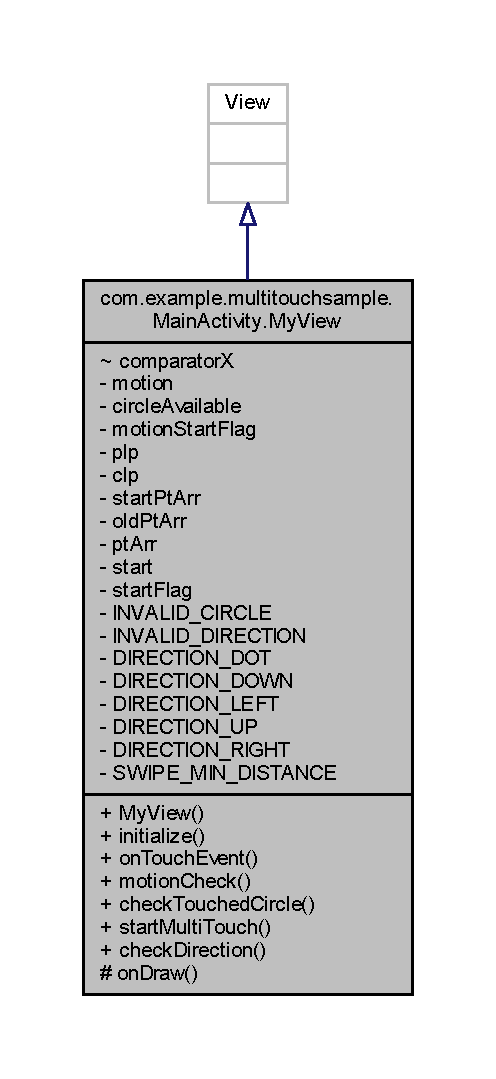
\includegraphics[width=238pt]{classcom_1_1example_1_1multitouchsample_1_1_main_activity_1_1_my_view__inherit__graph}
\end{center}
\end{figure}


Collaboration diagram for com.\+example.\+multitouchsample.\+Main\+Activity.\+My\+View\+:
\nopagebreak
\begin{figure}[H]
\begin{center}
\leavevmode
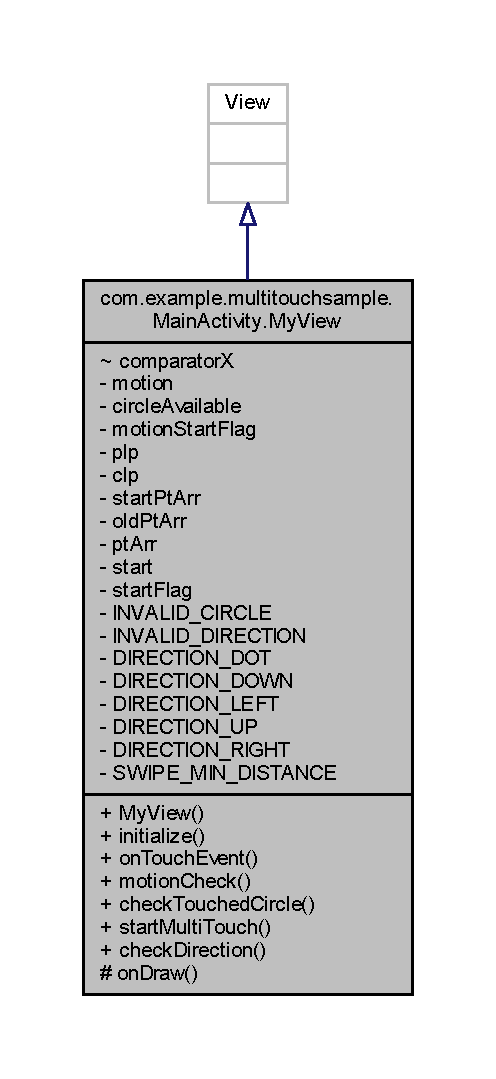
\includegraphics[width=238pt]{classcom_1_1example_1_1multitouchsample_1_1_main_activity_1_1_my_view__coll__graph}
\end{center}
\end{figure}
\subsection*{Classes}
\begin{DoxyCompactItemize}
\item 
class \hyperlink{classcom_1_1example_1_1multitouchsample_1_1_main_activity_1_1_my_view_1_1_circle_linked_with_pt_id}{Circle\+Linked\+With\+Pt\+Id}
\item 
class \hyperlink{classcom_1_1example_1_1multitouchsample_1_1_main_activity_1_1_my_view_1_1_pt_id_linked_with_pt_index}{Pt\+Id\+Linked\+With\+Pt\+Index}
\end{DoxyCompactItemize}
\subsection*{Public Member Functions}
\begin{DoxyCompactItemize}
\item 
\hyperlink{classcom_1_1example_1_1multitouchsample_1_1_main_activity_1_1_my_view_a5df70aa609ad47a649b0b342199ef69b}{My\+View} (Context context)
\item 
void \hyperlink{classcom_1_1example_1_1multitouchsample_1_1_main_activity_1_1_my_view_a228c403eab8cc3e845623b26e23c05d8}{initialize} ()
\begin{DoxyCompactList}\small\item\em Function information \+: Initialize function. \end{DoxyCompactList}\item 
boolean \hyperlink{classcom_1_1example_1_1multitouchsample_1_1_main_activity_1_1_my_view_ab2bf7ce103f9d65b6d677274d51a887e}{on\+Touch\+Event} (Motion\+Event e)
\item 
void \hyperlink{classcom_1_1example_1_1multitouchsample_1_1_main_activity_1_1_my_view_aee59904e43e35df3dd7684f22b7dc65d}{motion\+Check} ()
\begin{DoxyCompactList}\small\item\em Function information \+: Motion checking method. \end{DoxyCompactList}\item 
int \hyperlink{classcom_1_1example_1_1multitouchsample_1_1_main_activity_1_1_my_view_a98456bf5be1085790b22ea0179fa2892}{check\+Touched\+Circle} (int x, int y)
\begin{DoxyCompactList}\small\item\em Function information \+: Find touched circle. \end{DoxyCompactList}\item 
boolean \hyperlink{classcom_1_1example_1_1multitouchsample_1_1_main_activity_1_1_my_view_a98da479657a7dabe6b6dee15e39b5a98}{start\+Multi\+Touch} (Motion\+Event e)
\begin{DoxyCompactList}\small\item\em Function information \+: Start multi touch recognition. \end{DoxyCompactList}\item 
void \hyperlink{classcom_1_1example_1_1multitouchsample_1_1_main_activity_1_1_my_view_a6fbf678025aa07a8024eddeb5431b30c}{check\+Direction} (\hyperlink{classcom_1_1example_1_1multitouchsample_1_1_main_activity_1_1_my_view_1_1_pt_id_linked_with_pt_index}{Pt\+Id\+Linked\+With\+Pt\+Index} pp, Point\+F pt)
\begin{DoxyCompactList}\small\item\em Function information \+: Check the direction of movement of pointers. \end{DoxyCompactList}\end{DoxyCompactItemize}
\subsection*{Protected Member Functions}
\begin{DoxyCompactItemize}
\item 
void \hyperlink{classcom_1_1example_1_1multitouchsample_1_1_main_activity_1_1_my_view_a26704cac8a42993a73637404da71988e}{on\+Draw} (Canvas canvas)
\end{DoxyCompactItemize}
\subsection*{Private Attributes}
\begin{DoxyCompactItemize}
\item 
int\mbox{[}$\,$\mbox{]} \hyperlink{classcom_1_1example_1_1multitouchsample_1_1_main_activity_1_1_my_view_a3e8186596771c2fae1397b496be41230}{motion}
\item 
boolean\mbox{[}$\,$\mbox{]} \hyperlink{classcom_1_1example_1_1multitouchsample_1_1_main_activity_1_1_my_view_a5df7070a08705a7a8d8aa00a906fa767}{circle\+Available}
\item 
boolean \hyperlink{classcom_1_1example_1_1multitouchsample_1_1_main_activity_1_1_my_view_ab1da26ed65817fe5db4d0be4892ac4b2}{motion\+Start\+Flag}
\item 
Linked\+List$<$ \hyperlink{classcom_1_1example_1_1multitouchsample_1_1_main_activity_1_1_my_view_1_1_pt_id_linked_with_pt_index}{Pt\+Id\+Linked\+With\+Pt\+Index} $>$ \hyperlink{classcom_1_1example_1_1multitouchsample_1_1_main_activity_1_1_my_view_a594a2fb9e001c0cfa1aa538c903bc3f8}{plp}
\item 
Array\+List$<$ \hyperlink{classcom_1_1example_1_1multitouchsample_1_1_main_activity_1_1_my_view_1_1_circle_linked_with_pt_id}{Circle\+Linked\+With\+Pt\+Id} $>$ \hyperlink{classcom_1_1example_1_1multitouchsample_1_1_main_activity_1_1_my_view_a3bbc2d3fe569814080fe27c6c64eca77}{clp}
\item 
Array\+List$<$ Point\+F $>$ \hyperlink{classcom_1_1example_1_1multitouchsample_1_1_main_activity_1_1_my_view_a8e580a64440ed09158aa2bbc50ad4cf6}{start\+Pt\+Arr}
\item 
Array\+List$<$ Point\+F $>$ \hyperlink{classcom_1_1example_1_1multitouchsample_1_1_main_activity_1_1_my_view_abf78b5272ae2cffeed639bd024d2a642}{old\+Pt\+Arr}
\item 
Array\+List$<$ Point\+F $>$ \hyperlink{classcom_1_1example_1_1multitouchsample_1_1_main_activity_1_1_my_view_ab2213518b7234955478ef54ebdd1db22}{pt\+Arr}
\item 
boolean \hyperlink{classcom_1_1example_1_1multitouchsample_1_1_main_activity_1_1_my_view_a45f874e10d05217f17e21ebee2f636ea}{start}
\item 
boolean \hyperlink{classcom_1_1example_1_1multitouchsample_1_1_main_activity_1_1_my_view_a10816f1798f68acf937c930b526b112d}{start\+Flag}
\end{DoxyCompactItemize}
\subsection*{Static Private Attributes}
\begin{DoxyCompactItemize}
\item 
static final int \hyperlink{classcom_1_1example_1_1multitouchsample_1_1_main_activity_1_1_my_view_a90558b5e086112625e29f3941b1444d8}{I\+N\+V\+A\+L\+I\+D\+\_\+\+C\+I\+R\+C\+L\+E} = -\/1
\item 
static final int \hyperlink{classcom_1_1example_1_1multitouchsample_1_1_main_activity_1_1_my_view_a1b17ab3dd378a4846a8de05a58fce3db}{I\+N\+V\+A\+L\+I\+D\+\_\+\+D\+I\+R\+E\+C\+T\+I\+O\+N} = -\/1
\item 
static final int \hyperlink{classcom_1_1example_1_1multitouchsample_1_1_main_activity_1_1_my_view_ad91938a7ac9667ccd247a072f338a2de}{D\+I\+R\+E\+C\+T\+I\+O\+N\+\_\+\+D\+O\+T} = 0
\item 
static final int \hyperlink{classcom_1_1example_1_1multitouchsample_1_1_main_activity_1_1_my_view_afc3ae0a948391b36141f78c515622217}{D\+I\+R\+E\+C\+T\+I\+O\+N\+\_\+\+D\+O\+W\+N} = 1
\item 
static final int \hyperlink{classcom_1_1example_1_1multitouchsample_1_1_main_activity_1_1_my_view_aad2a71c46e7cad809a27eb9c4c2600d9}{D\+I\+R\+E\+C\+T\+I\+O\+N\+\_\+\+L\+E\+F\+T} = 2
\item 
static final int \hyperlink{classcom_1_1example_1_1multitouchsample_1_1_main_activity_1_1_my_view_a43c4159b9b295cfea731211ac614fc0b}{D\+I\+R\+E\+C\+T\+I\+O\+N\+\_\+\+U\+P} = 3
\item 
static final int \hyperlink{classcom_1_1example_1_1multitouchsample_1_1_main_activity_1_1_my_view_a2d1dd293bf4c64feec7de128ef21739e}{D\+I\+R\+E\+C\+T\+I\+O\+N\+\_\+\+R\+I\+G\+H\+T} = 4
\item 
static final int \hyperlink{classcom_1_1example_1_1multitouchsample_1_1_main_activity_1_1_my_view_a677194aa1ca850fc0e716d725f691ba1}{S\+W\+I\+P\+E\+\_\+\+M\+I\+N\+\_\+\+D\+I\+S\+T\+A\+N\+C\+E} = 140
\end{DoxyCompactItemize}


\subsection{Detailed Description}


Definition at line 30 of file Main\+Activity.\+java.



\subsection{Constructor \& Destructor Documentation}
\hypertarget{classcom_1_1example_1_1multitouchsample_1_1_main_activity_1_1_my_view_a5df70aa609ad47a649b0b342199ef69b}{}\index{com\+::example\+::multitouchsample\+::\+Main\+Activity\+::\+My\+View@{com\+::example\+::multitouchsample\+::\+Main\+Activity\+::\+My\+View}!My\+View@{My\+View}}
\index{My\+View@{My\+View}!com\+::example\+::multitouchsample\+::\+Main\+Activity\+::\+My\+View@{com\+::example\+::multitouchsample\+::\+Main\+Activity\+::\+My\+View}}
\subsubsection[{My\+View}]{\setlength{\rightskip}{0pt plus 5cm}com.\+example.\+multitouchsample.\+Main\+Activity.\+My\+View.\+My\+View (
\begin{DoxyParamCaption}
\item[{Context}]{context}
\end{DoxyParamCaption}
)}\label{classcom_1_1example_1_1multitouchsample_1_1_main_activity_1_1_my_view_a5df70aa609ad47a649b0b342199ef69b}


Definition at line 42 of file Main\+Activity.\+java.


\begin{DoxyCode}
43         \{
44             super(context);
45             \hyperlink{classcom_1_1example_1_1multitouchsample_1_1_main_activity_1_1_my_view_a228c403eab8cc3e845623b26e23c05d8}{initialize}();
46         \}
\end{DoxyCode}


Here is the call graph for this function\+:
\nopagebreak
\begin{figure}[H]
\begin{center}
\leavevmode
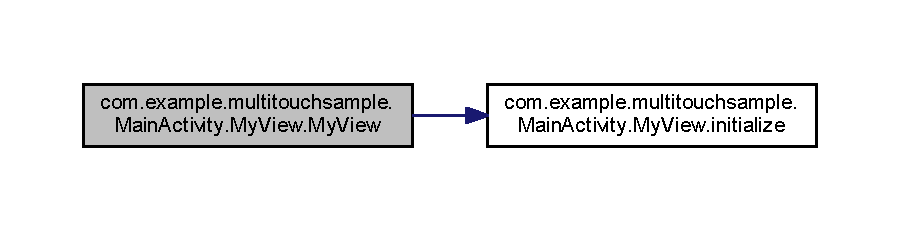
\includegraphics[width=350pt]{classcom_1_1example_1_1multitouchsample_1_1_main_activity_1_1_my_view_a5df70aa609ad47a649b0b342199ef69b_cgraph}
\end{center}
\end{figure}




\subsection{Member Function Documentation}
\hypertarget{classcom_1_1example_1_1multitouchsample_1_1_main_activity_1_1_my_view_a6fbf678025aa07a8024eddeb5431b30c}{}\index{com\+::example\+::multitouchsample\+::\+Main\+Activity\+::\+My\+View@{com\+::example\+::multitouchsample\+::\+Main\+Activity\+::\+My\+View}!check\+Direction@{check\+Direction}}
\index{check\+Direction@{check\+Direction}!com\+::example\+::multitouchsample\+::\+Main\+Activity\+::\+My\+View@{com\+::example\+::multitouchsample\+::\+Main\+Activity\+::\+My\+View}}
\subsubsection[{check\+Direction}]{\setlength{\rightskip}{0pt plus 5cm}com.\+example.\+multitouchsample.\+Main\+Activity.\+My\+View.\+check\+Direction (
\begin{DoxyParamCaption}
\item[{{\bf Pt\+Id\+Linked\+With\+Pt\+Index}}]{pp, }
\item[{Point\+F}]{pt}
\end{DoxyParamCaption}
)}\label{classcom_1_1example_1_1multitouchsample_1_1_main_activity_1_1_my_view_a6fbf678025aa07a8024eddeb5431b30c}


Function information \+: Check the direction of movement of pointers. 

\begin{DoxyRemark}{Remarks}

\begin{DoxyItemize}
\item Description \+: Calculate the moved distances of pointers and save them in \textquotesingle{}motion\textquotesingle{} array. 
\end{DoxyItemize}
\end{DoxyRemark}

\begin{DoxyParams}{Parameters}
{\em pp} & \+: List of class which has Pointer I\+D and Pointer Index to link them. \\
\hline
{\em pt} & \+: Grid of currently moving pointer.\\
\hline
\end{DoxyParams}

\begin{DoxyCode}
\textcolor{comment}{// core code}
\end{DoxyCode}
 

Definition at line 508 of file Main\+Activity.\+java.


\begin{DoxyCode}
509         \{
510             CircleLinkedWithPtId cp = \textcolor{keyword}{new} CircleLinkedWithPtId();
511             \textcolor{keywordflow}{for}(\textcolor{keywordtype}{int} i=0; i<5; i++)
512             \{
513                 \textcolor{keywordflow}{if}(\hyperlink{classcom_1_1example_1_1multitouchsample_1_1_main_activity_1_1_my_view_a3bbc2d3fe569814080fe27c6c64eca77}{clp}.size() <= i)
514                     \textcolor{keywordflow}{return};
515                 cp = \hyperlink{classcom_1_1example_1_1multitouchsample_1_1_main_activity_1_1_my_view_a3bbc2d3fe569814080fe27c6c64eca77}{clp}.get(i);
516                 \textcolor{keywordflow}{if}(pp.pointerId == cp.pointerId)
517                     \textcolor{keywordflow}{break};
518             \}
519             
520             PointF oldPt = \textcolor{keyword}{new} PointF();
521             \textcolor{keywordtype}{int} circleNum = -1;
522             \textcolor{keywordflow}{for}(\textcolor{keywordtype}{int} i=0; i<5; i++)
523             \{
524                 \textcolor{keywordflow}{if}(\hyperlink{classcom_1_1example_1_1multitouchsample_1_1_main_activity_1_1_my_view_abf78b5272ae2cffeed639bd024d2a642}{oldPtArr}.size() <= i)
525                     \textcolor{keywordflow}{break};
526                 oldPt = \hyperlink{classcom_1_1example_1_1multitouchsample_1_1_main_activity_1_1_my_view_abf78b5272ae2cffeed639bd024d2a642}{oldPtArr}.get(i);
527                 circleNum = \hyperlink{classcom_1_1example_1_1multitouchsample_1_1_main_activity_1_1_my_view_a98456bf5be1085790b22ea0179fa2892}{checkTouchedCircle}((\textcolor{keywordtype}{int})oldPt.x, (\textcolor{keywordtype}{int})oldPt.y);
528                 \textcolor{keywordflow}{if}(cp.circleNum == circleNum)
529                     \textcolor{keywordflow}{break};
530             \}
531             \textcolor{keywordflow}{if}(circleNum == -1) \textcolor{keywordflow}{return};
532             
533             \textcolor{keywordtype}{float} distanceX = oldPt.x - pt.x;
534             \textcolor{keywordtype}{float} distanceY = oldPt.y - pt.y;
535             
536             \textcolor{keywordflow}{if}( Math.abs(distanceX) < \hyperlink{classcom_1_1example_1_1multitouchsample_1_1_main_activity_1_1_my_view_a677194aa1ca850fc0e716d725f691ba1}{SWIPE\_MIN\_DISTANCE} && Math.abs(distanceY) < 
      \hyperlink{classcom_1_1example_1_1multitouchsample_1_1_main_activity_1_1_my_view_a677194aa1ca850fc0e716d725f691ba1}{SWIPE\_MIN\_DISTANCE} )
537                 \hyperlink{classcom_1_1example_1_1multitouchsample_1_1_main_activity_1_1_my_view_a3e8186596771c2fae1397b496be41230}{motion}[circleNum-1] = \hyperlink{classcom_1_1example_1_1multitouchsample_1_1_main_activity_1_1_my_view_ad91938a7ac9667ccd247a072f338a2de}{DIRECTION\_DOT};
538             \textcolor{keywordflow}{else} \textcolor{keywordflow}{if}( Math.abs(distanceX) > \hyperlink{classcom_1_1example_1_1multitouchsample_1_1_main_activity_1_1_my_view_a677194aa1ca850fc0e716d725f691ba1}{SWIPE\_MIN\_DISTANCE} && Math.abs(distanceY) > 
      \hyperlink{classcom_1_1example_1_1multitouchsample_1_1_main_activity_1_1_my_view_a677194aa1ca850fc0e716d725f691ba1}{SWIPE\_MIN\_DISTANCE} )
539                 \hyperlink{classcom_1_1example_1_1multitouchsample_1_1_main_activity_1_1_my_view_a3e8186596771c2fae1397b496be41230}{motion}[circleNum-1] = \hyperlink{classcom_1_1example_1_1multitouchsample_1_1_main_activity_1_1_my_view_a1b17ab3dd378a4846a8de05a58fce3db}{INVALID\_DIRECTION};
540             \textcolor{keywordflow}{else} \textcolor{keywordflow}{if}( Math.abs(distanceX) > \hyperlink{classcom_1_1example_1_1multitouchsample_1_1_main_activity_1_1_my_view_a677194aa1ca850fc0e716d725f691ba1}{SWIPE\_MIN\_DISTANCE} && distanceX > 0)
541                 \hyperlink{classcom_1_1example_1_1multitouchsample_1_1_main_activity_1_1_my_view_a3e8186596771c2fae1397b496be41230}{motion}[circleNum-1] = \hyperlink{classcom_1_1example_1_1multitouchsample_1_1_main_activity_1_1_my_view_aad2a71c46e7cad809a27eb9c4c2600d9}{DIRECTION\_LEFT};
542             \textcolor{keywordflow}{else} \textcolor{keywordflow}{if}( Math.abs(distanceX) > \hyperlink{classcom_1_1example_1_1multitouchsample_1_1_main_activity_1_1_my_view_a677194aa1ca850fc0e716d725f691ba1}{SWIPE\_MIN\_DISTANCE} && distanceX < 0)
543                 \hyperlink{classcom_1_1example_1_1multitouchsample_1_1_main_activity_1_1_my_view_a3e8186596771c2fae1397b496be41230}{motion}[circleNum-1] = \hyperlink{classcom_1_1example_1_1multitouchsample_1_1_main_activity_1_1_my_view_a2d1dd293bf4c64feec7de128ef21739e}{DIRECTION\_RIGHT};
544             \textcolor{keywordflow}{else} \textcolor{keywordflow}{if}( Math.abs(distanceY) > \hyperlink{classcom_1_1example_1_1multitouchsample_1_1_main_activity_1_1_my_view_a677194aa1ca850fc0e716d725f691ba1}{SWIPE\_MIN\_DISTANCE} && distanceY < 0)
545                 \hyperlink{classcom_1_1example_1_1multitouchsample_1_1_main_activity_1_1_my_view_a3e8186596771c2fae1397b496be41230}{motion}[circleNum-1] = \hyperlink{classcom_1_1example_1_1multitouchsample_1_1_main_activity_1_1_my_view_afc3ae0a948391b36141f78c515622217}{DIRECTION\_DOWN};
546             \textcolor{keywordflow}{else} \textcolor{keywordflow}{if}( Math.abs(distanceY) > \hyperlink{classcom_1_1example_1_1multitouchsample_1_1_main_activity_1_1_my_view_a677194aa1ca850fc0e716d725f691ba1}{SWIPE\_MIN\_DISTANCE} && distanceY > 0)
547                 \hyperlink{classcom_1_1example_1_1multitouchsample_1_1_main_activity_1_1_my_view_a3e8186596771c2fae1397b496be41230}{motion}[circleNum-1] = \hyperlink{classcom_1_1example_1_1multitouchsample_1_1_main_activity_1_1_my_view_a43c4159b9b295cfea731211ac614fc0b}{DIRECTION\_UP};
548             \textcolor{keywordflow}{else}
549                 \hyperlink{classcom_1_1example_1_1multitouchsample_1_1_main_activity_1_1_my_view_a3e8186596771c2fae1397b496be41230}{motion}[circleNum-1] = \hyperlink{classcom_1_1example_1_1multitouchsample_1_1_main_activity_1_1_my_view_a1b17ab3dd378a4846a8de05a58fce3db}{INVALID\_DIRECTION};
550         \}
\end{DoxyCode}


Here is the call graph for this function\+:
\nopagebreak
\begin{figure}[H]
\begin{center}
\leavevmode
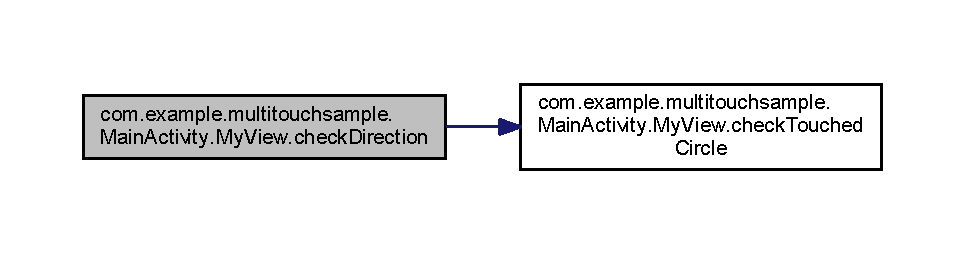
\includegraphics[width=350pt]{classcom_1_1example_1_1multitouchsample_1_1_main_activity_1_1_my_view_a6fbf678025aa07a8024eddeb5431b30c_cgraph}
\end{center}
\end{figure}




Here is the caller graph for this function\+:
\nopagebreak
\begin{figure}[H]
\begin{center}
\leavevmode
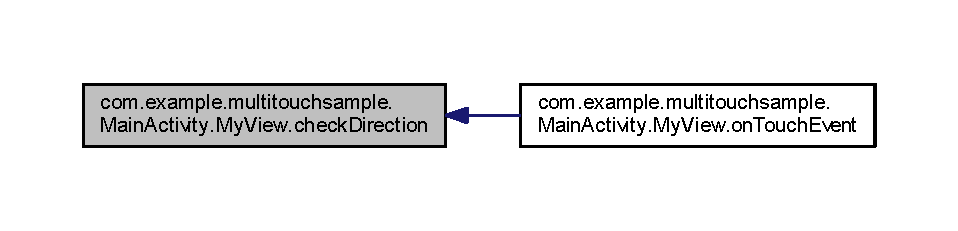
\includegraphics[width=350pt]{classcom_1_1example_1_1multitouchsample_1_1_main_activity_1_1_my_view_a6fbf678025aa07a8024eddeb5431b30c_icgraph}
\end{center}
\end{figure}


\hypertarget{classcom_1_1example_1_1multitouchsample_1_1_main_activity_1_1_my_view_a98456bf5be1085790b22ea0179fa2892}{}\index{com\+::example\+::multitouchsample\+::\+Main\+Activity\+::\+My\+View@{com\+::example\+::multitouchsample\+::\+Main\+Activity\+::\+My\+View}!check\+Touched\+Circle@{check\+Touched\+Circle}}
\index{check\+Touched\+Circle@{check\+Touched\+Circle}!com\+::example\+::multitouchsample\+::\+Main\+Activity\+::\+My\+View@{com\+::example\+::multitouchsample\+::\+Main\+Activity\+::\+My\+View}}
\subsubsection[{check\+Touched\+Circle}]{\setlength{\rightskip}{0pt plus 5cm}com.\+example.\+multitouchsample.\+Main\+Activity.\+My\+View.\+check\+Touched\+Circle (
\begin{DoxyParamCaption}
\item[{int}]{x, }
\item[{int}]{y}
\end{DoxyParamCaption}
)}\label{classcom_1_1example_1_1multitouchsample_1_1_main_activity_1_1_my_view_a98456bf5be1085790b22ea0179fa2892}


Function information \+: Find touched circle. 

\begin{DoxyRemark}{Remarks}

\begin{DoxyItemize}
\item Description \+: This method will check which circle is touched 
\end{DoxyItemize}
\end{DoxyRemark}

\begin{DoxyParams}{Parameters}
{\em x} & x grid of touched point \\
\hline
{\em y} & y grid of touched point \\
\hline
\end{DoxyParams}
\begin{DoxyReturn}{Returns}
Returns touched circle number. If any of circle is touched, return -\/1.
\end{DoxyReturn}

\begin{DoxyCode}
\textcolor{comment}{// core code}
\end{DoxyCode}
 

Definition at line 437 of file Main\+Activity.\+java.


\begin{DoxyCode}
438         \{
439             \textcolor{keywordtype}{int} index=0;
440             \textcolor{keywordflow}{for}(PointF spt : \hyperlink{classcom_1_1example_1_1multitouchsample_1_1_main_activity_1_1_my_view_a8e580a64440ed09158aa2bbc50ad4cf6}{startPtArr})
441             \{
442                 index++;
443                 \textcolor{keywordflow}{if}( (Math.abs((\textcolor{keywordtype}{int})spt.x - x) < 180) && (Math.abs((\textcolor{keywordtype}{int})spt.y - y) < 140) )
444                     \textcolor{keywordflow}{return} index;
445             \}
446             \textcolor{keywordflow}{return} -1;
447         \}
\end{DoxyCode}


Here is the caller graph for this function\+:
\nopagebreak
\begin{figure}[H]
\begin{center}
\leavevmode
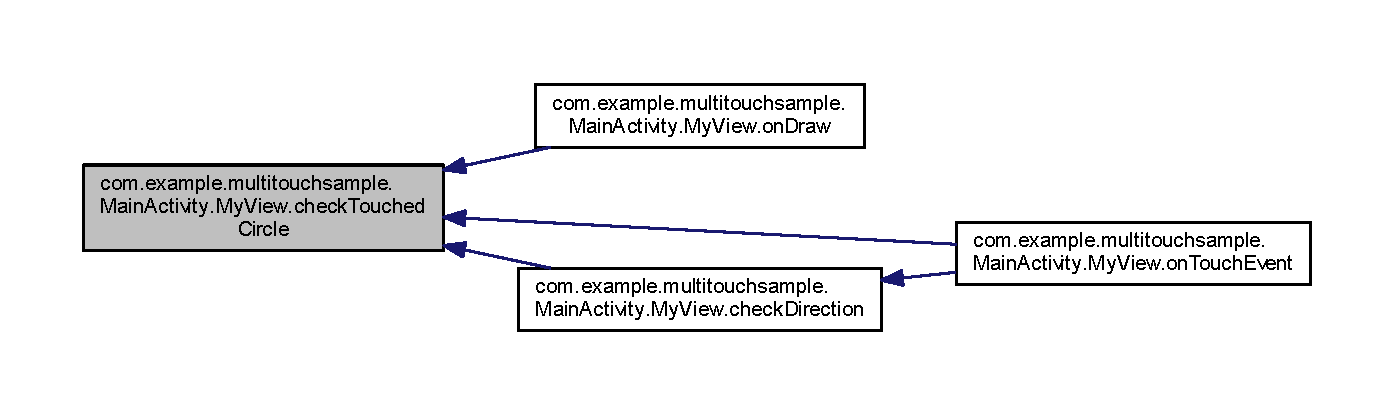
\includegraphics[width=350pt]{classcom_1_1example_1_1multitouchsample_1_1_main_activity_1_1_my_view_a98456bf5be1085790b22ea0179fa2892_icgraph}
\end{center}
\end{figure}


\hypertarget{classcom_1_1example_1_1multitouchsample_1_1_main_activity_1_1_my_view_a228c403eab8cc3e845623b26e23c05d8}{}\index{com\+::example\+::multitouchsample\+::\+Main\+Activity\+::\+My\+View@{com\+::example\+::multitouchsample\+::\+Main\+Activity\+::\+My\+View}!initialize@{initialize}}
\index{initialize@{initialize}!com\+::example\+::multitouchsample\+::\+Main\+Activity\+::\+My\+View@{com\+::example\+::multitouchsample\+::\+Main\+Activity\+::\+My\+View}}
\subsubsection[{initialize}]{\setlength{\rightskip}{0pt plus 5cm}com.\+example.\+multitouchsample.\+Main\+Activity.\+My\+View.\+initialize (
\begin{DoxyParamCaption}
{}
\end{DoxyParamCaption}
)}\label{classcom_1_1example_1_1multitouchsample_1_1_main_activity_1_1_my_view_a228c403eab8cc3e845623b26e23c05d8}


Function information \+: Initialize function. 

\begin{DoxyRemark}{Remarks}

\begin{DoxyItemize}
\item Description \+: Initialize all variables and lists
\end{DoxyItemize}
\end{DoxyRemark}

\begin{DoxyCode}
\textcolor{comment}{// core code}
\end{DoxyCode}
 

Definition at line 151 of file Main\+Activity.\+java.


\begin{DoxyCode}
152         \{
153             \hyperlink{classcom_1_1example_1_1multitouchsample_1_1_main_activity_1_1_my_view_a10816f1798f68acf937c930b526b112d}{startFlag} = \textcolor{keyword}{false};
154             \hyperlink{classcom_1_1example_1_1multitouchsample_1_1_main_activity_1_1_my_view_a45f874e10d05217f17e21ebee2f636ea}{start} = \textcolor{keyword}{false};
155             \hyperlink{classcom_1_1example_1_1multitouchsample_1_1_main_activity_1_1_my_view_ab1da26ed65817fe5db4d0be4892ac4b2}{motionStartFlag} = \textcolor{keyword}{false};
156             \hyperlink{classcom_1_1example_1_1multitouchsample_1_1_main_activity_1_1_my_view_a3e8186596771c2fae1397b496be41230}{motion} = \textcolor{keyword}{new} \textcolor{keywordtype}{int}[5];
157             \hyperlink{classcom_1_1example_1_1multitouchsample_1_1_main_activity_1_1_my_view_a5df7070a08705a7a8d8aa00a906fa767}{circleAvailable} = \textcolor{keyword}{new} \textcolor{keywordtype}{boolean}[5];
158             \textcolor{keywordflow}{for}(\textcolor{keywordtype}{int} i=0; i<5; i++)
159                 \hyperlink{classcom_1_1example_1_1multitouchsample_1_1_main_activity_1_1_my_view_a5df7070a08705a7a8d8aa00a906fa767}{circleAvailable}[i] = \textcolor{keyword}{true};
160             
161             \hyperlink{classcom_1_1example_1_1multitouchsample_1_1_main_activity_1_1_my_view_a594a2fb9e001c0cfa1aa538c903bc3f8}{plp} = \textcolor{keyword}{new} LinkedList<PtIdLinkedWithPtIndex>();
162             \hyperlink{classcom_1_1example_1_1multitouchsample_1_1_main_activity_1_1_my_view_a3bbc2d3fe569814080fe27c6c64eca77}{clp} = \textcolor{keyword}{new} ArrayList<CircleLinkedWithPtId>();
163             
164             \hyperlink{classcom_1_1example_1_1multitouchsample_1_1_main_activity_1_1_my_view_a8e580a64440ed09158aa2bbc50ad4cf6}{startPtArr} = \textcolor{keyword}{new} ArrayList<PointF>();
165             \hyperlink{classcom_1_1example_1_1multitouchsample_1_1_main_activity_1_1_my_view_abf78b5272ae2cffeed639bd024d2a642}{oldPtArr} = \textcolor{keyword}{new} ArrayList<PointF>();
166             \hyperlink{classcom_1_1example_1_1multitouchsample_1_1_main_activity_1_1_my_view_ab2213518b7234955478ef54ebdd1db22}{ptArr} = \textcolor{keyword}{new} ArrayList<PointF>();
167             
168             \hyperlink{classcom_1_1example_1_1multitouchsample_1_1_main_activity_1_1_my_view_a594a2fb9e001c0cfa1aa538c903bc3f8}{plp}.clear();
169             clp.clear();
170             
171             startPtArr.clear();
172             oldPtArr.clear();
173             ptArr.clear();
174         \}
\end{DoxyCode}


Here is the caller graph for this function\+:
\nopagebreak
\begin{figure}[H]
\begin{center}
\leavevmode
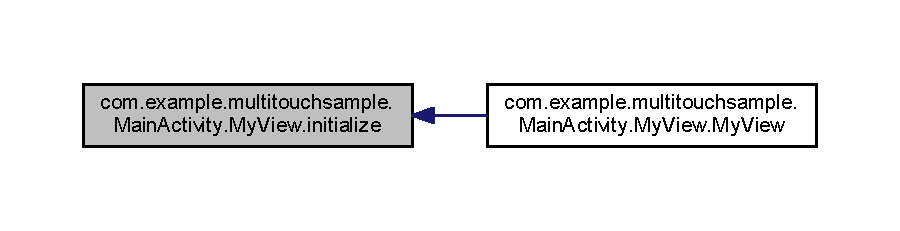
\includegraphics[width=350pt]{classcom_1_1example_1_1multitouchsample_1_1_main_activity_1_1_my_view_a228c403eab8cc3e845623b26e23c05d8_icgraph}
\end{center}
\end{figure}


\hypertarget{classcom_1_1example_1_1multitouchsample_1_1_main_activity_1_1_my_view_aee59904e43e35df3dd7684f22b7dc65d}{}\index{com\+::example\+::multitouchsample\+::\+Main\+Activity\+::\+My\+View@{com\+::example\+::multitouchsample\+::\+Main\+Activity\+::\+My\+View}!motion\+Check@{motion\+Check}}
\index{motion\+Check@{motion\+Check}!com\+::example\+::multitouchsample\+::\+Main\+Activity\+::\+My\+View@{com\+::example\+::multitouchsample\+::\+Main\+Activity\+::\+My\+View}}
\subsubsection[{motion\+Check}]{\setlength{\rightskip}{0pt plus 5cm}com.\+example.\+multitouchsample.\+Main\+Activity.\+My\+View.\+motion\+Check (
\begin{DoxyParamCaption}
{}
\end{DoxyParamCaption}
)}\label{classcom_1_1example_1_1multitouchsample_1_1_main_activity_1_1_my_view_aee59904e43e35df3dd7684f22b7dc65d}


Function information \+: Motion checking method. 

\begin{DoxyRemark}{Remarks}

\begin{DoxyItemize}
\item Description \+: In A\+C\+T\+I\+O\+N\+\_\+\+U\+P motion event, this method will be called.~\newline
 Checks motion array and check motion of each pointer.~\newline

\begin{DoxyCode}
\textcolor{comment}{// core code}
\end{DoxyCode}
 
\end{DoxyItemize}
\end{DoxyRemark}


Definition at line 378 of file Main\+Activity.\+java.


\begin{DoxyCode}
379         \{
380             String command = \textcolor{stringliteral}{""};
381             \textcolor{keywordflow}{for}(\textcolor{keywordtype}{int} i=0; i<5; i++)
382             \{
383                 \textcolor{keywordflow}{if}(\hyperlink{classcom_1_1example_1_1multitouchsample_1_1_main_activity_1_1_my_view_a3e8186596771c2fae1397b496be41230}{motion}[i] != -1)
384                 \{
385                     \textcolor{keywordflow}{switch}(\hyperlink{classcom_1_1example_1_1multitouchsample_1_1_main_activity_1_1_my_view_a3e8186596771c2fae1397b496be41230}{motion}[i])
386                     \{
387                         \textcolor{keywordflow}{case} \hyperlink{classcom_1_1example_1_1multitouchsample_1_1_main_activity_1_1_my_view_ad91938a7ac9667ccd247a072f338a2de}{DIRECTION\_DOT} :
388                         \{
389                             Log.d(\textcolor{stringliteral}{"UP"}, \textcolor{stringliteral}{"circleIndex : "} + (i+1) + \textcolor{stringliteral}{"| Dir) DOT"});
390                             command += \textcolor{stringliteral}{"circleIndex : "} + (i+1) + \textcolor{stringliteral}{"| Dir) DOT\(\backslash\)n"};
391                             \textcolor{keywordflow}{break};
392                         \}
393                         \textcolor{keywordflow}{case} \hyperlink{classcom_1_1example_1_1multitouchsample_1_1_main_activity_1_1_my_view_a43c4159b9b295cfea731211ac614fc0b}{DIRECTION\_UP} :
394                         \{
395                             Log.d(\textcolor{stringliteral}{"UP"}, \textcolor{stringliteral}{"circleIndex : "} + (i+1) + \textcolor{stringliteral}{"| Dir) UP"});
396                             command += \textcolor{stringliteral}{"circleIndex : "} + (i+1) + \textcolor{stringliteral}{"| Dir) UP\(\backslash\)n"};
397                             \textcolor{keywordflow}{break};
398                         \}
399                         \textcolor{keywordflow}{case} \hyperlink{classcom_1_1example_1_1multitouchsample_1_1_main_activity_1_1_my_view_afc3ae0a948391b36141f78c515622217}{DIRECTION\_DOWN} :
400                         \{
401                             Log.d(\textcolor{stringliteral}{"UP"}, \textcolor{stringliteral}{"circleIndex : "} + (i+1) + \textcolor{stringliteral}{"| Dir) DOWN"});
402                             command += \textcolor{stringliteral}{"circleIndex : "} + (i+1) + \textcolor{stringliteral}{"| Dir) DOWN\(\backslash\)n"};
403                             \textcolor{keywordflow}{break};
404                         \}
405                         \textcolor{keywordflow}{case} \hyperlink{classcom_1_1example_1_1multitouchsample_1_1_main_activity_1_1_my_view_aad2a71c46e7cad809a27eb9c4c2600d9}{DIRECTION\_LEFT} :
406                         \{
407                             Log.d(\textcolor{stringliteral}{"UP"}, \textcolor{stringliteral}{"circleIndex : "} + (i+1) + \textcolor{stringliteral}{"| Dir) LEFT"});
408                             command += \textcolor{stringliteral}{"circleIndex : "} + (i+1) + \textcolor{stringliteral}{"| Dir) LEFT\(\backslash\)n"};
409                             \textcolor{keywordflow}{break};
410                         \}
411                         \textcolor{keywordflow}{case} \hyperlink{classcom_1_1example_1_1multitouchsample_1_1_main_activity_1_1_my_view_a2d1dd293bf4c64feec7de128ef21739e}{DIRECTION\_RIGHT} :
412                         \{
413                             Log.d(\textcolor{stringliteral}{"UP"}, \textcolor{stringliteral}{"circleIndex : "} + (i+1) + \textcolor{stringliteral}{"| Dir) RIGHT"});
414                             command += \textcolor{stringliteral}{"circleIndex : "} + (i+1) + \textcolor{stringliteral}{"| Dir) RIGHT\(\backslash\)n"};
415                         \}
416                     \}\textcolor{comment}{//switch end}
417                 \}\textcolor{comment}{//motion check if end}
418             \}\textcolor{comment}{//motion check for end}
419             Log.d(\textcolor{stringliteral}{"Motion End"}, \textcolor{stringliteral}{"------------------------------"});
420             \textcolor{keywordflow}{if}(!command.equals(\textcolor{stringliteral}{""}))
421                 Toast.makeText(\hyperlink{classcom_1_1example_1_1multitouchsample_1_1_main_activity_a55ac0e8368b828f2e73446810af25a24}{ctx}, command, android.widget.Toast.LENGTH\_SHORT).show();
422         \}
\end{DoxyCode}


Here is the caller graph for this function\+:
\nopagebreak
\begin{figure}[H]
\begin{center}
\leavevmode
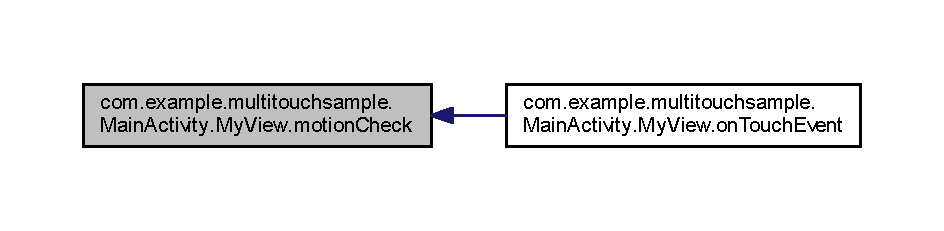
\includegraphics[width=350pt]{classcom_1_1example_1_1multitouchsample_1_1_main_activity_1_1_my_view_aee59904e43e35df3dd7684f22b7dc65d_icgraph}
\end{center}
\end{figure}


\hypertarget{classcom_1_1example_1_1multitouchsample_1_1_main_activity_1_1_my_view_a26704cac8a42993a73637404da71988e}{}\index{com\+::example\+::multitouchsample\+::\+Main\+Activity\+::\+My\+View@{com\+::example\+::multitouchsample\+::\+Main\+Activity\+::\+My\+View}!on\+Draw@{on\+Draw}}
\index{on\+Draw@{on\+Draw}!com\+::example\+::multitouchsample\+::\+Main\+Activity\+::\+My\+View@{com\+::example\+::multitouchsample\+::\+Main\+Activity\+::\+My\+View}}
\subsubsection[{on\+Draw}]{\setlength{\rightskip}{0pt plus 5cm}void com.\+example.\+multitouchsample.\+Main\+Activity.\+My\+View.\+on\+Draw (
\begin{DoxyParamCaption}
\item[{Canvas}]{canvas}
\end{DoxyParamCaption}
)\hspace{0.3cm}{\ttfamily [protected]}}\label{classcom_1_1example_1_1multitouchsample_1_1_main_activity_1_1_my_view_a26704cac8a42993a73637404da71988e}


Definition at line 185 of file Main\+Activity.\+java.


\begin{DoxyCode}
186         \{
187             Paint pnt = \textcolor{keyword}{new} Paint();
188             canvas.drawColor(Color.WHITE);
189             pnt.setTextSize(64.0f);         
190             
191             \textcolor{comment}{/* standard position */}
192             \textcolor{keywordflow}{if}(\hyperlink{classcom_1_1example_1_1multitouchsample_1_1_main_activity_1_1_my_view_a8e580a64440ed09158aa2bbc50ad4cf6}{startPtArr}.isEmpty())
193                 \textcolor{keywordflow}{return};
194             \textcolor{keywordtype}{int} index=0;
195             \textcolor{keywordflow}{for}(PointF spt : \hyperlink{classcom_1_1example_1_1multitouchsample_1_1_main_activity_1_1_my_view_a8e580a64440ed09158aa2bbc50ad4cf6}{startPtArr})
196             \{
197                 index++;
198                 pnt.setColor(Color.BLACK);
199                 pnt.setStyle(Paint.Style.STROKE);
200                 pnt.setStrokeWidth(1);
201                 canvas.drawCircle(spt.x,spt.y, 140, pnt);
202 
203                 pnt.setStyle(Paint.Style.FILL);
204                 canvas.drawText(String.valueOf(index),spt.x,spt.y-114,pnt);
205             \}
206             
207             \textcolor{comment}{/* down event position */}
208             \textcolor{keywordflow}{if}(!\hyperlink{classcom_1_1example_1_1multitouchsample_1_1_main_activity_1_1_my_view_abf78b5272ae2cffeed639bd024d2a642}{oldPtArr}.isEmpty())
209             \{
210                 \textcolor{keywordflow}{for} (PointF pt : \hyperlink{classcom_1_1example_1_1multitouchsample_1_1_main_activity_1_1_my_view_abf78b5272ae2cffeed639bd024d2a642}{oldPtArr})
211                 \{
212                     \textcolor{keywordtype}{int} circleNum = \hyperlink{classcom_1_1example_1_1multitouchsample_1_1_main_activity_1_1_my_view_a98456bf5be1085790b22ea0179fa2892}{checkTouchedCircle}((\textcolor{keywordtype}{int})pt.x, (\textcolor{keywordtype}{int})pt.y);
213                     pnt.setStyle(Paint.Style.STROKE);
214                     canvas.drawCircle(pt.x,pt.y, 100, pnt);
215     
216                     pnt.setStyle(Paint.Style.FILL);
217                     canvas.drawText(String.valueOf(circleNum),pt.x,pt.y-114,pnt);
218                 \}
219             \}
220             
221             \textcolor{comment}{/* current finger */}
222             index=0;
223             \textcolor{keywordflow}{if}(!\hyperlink{classcom_1_1example_1_1multitouchsample_1_1_main_activity_1_1_my_view_ab2213518b7234955478ef54ebdd1db22}{ptArr}.isEmpty() && !\hyperlink{classcom_1_1example_1_1multitouchsample_1_1_main_activity_1_1_my_view_a594a2fb9e001c0cfa1aa538c903bc3f8}{plp}.isEmpty() && !\hyperlink{classcom_1_1example_1_1multitouchsample_1_1_main_activity_1_1_my_view_a3bbc2d3fe569814080fe27c6c64eca77}{clp}.isEmpty())
224             \{           
225                 \textcolor{keywordflow}{for} (PointF pt : \hyperlink{classcom_1_1example_1_1multitouchsample_1_1_main_activity_1_1_my_view_ab2213518b7234955478ef54ebdd1db22}{ptArr})
226                 \{
227                     \textcolor{keywordtype}{int} pointerId = \hyperlink{classcom_1_1example_1_1multitouchsample_1_1_main_activity_1_1_my_view_a594a2fb9e001c0cfa1aa538c903bc3f8}{plp}.get(index++).pointerId;
228                     \textcolor{keywordflow}{if}(pointerId >= \hyperlink{classcom_1_1example_1_1multitouchsample_1_1_main_activity_1_1_my_view_a3bbc2d3fe569814080fe27c6c64eca77}{clp}.size())
229                         \textcolor{keywordflow}{break};                  
230                     \textcolor{keywordtype}{int} circleNum = \hyperlink{classcom_1_1example_1_1multitouchsample_1_1_main_activity_1_1_my_view_a3bbc2d3fe569814080fe27c6c64eca77}{clp}.get(pointerId).circleNum;
231                     
232                     pnt.setStyle(Paint.Style.STROKE);
233                     canvas.drawCircle(pt.x,pt.y, 100, pnt);
234     
235                     pnt.setStyle(Paint.Style.FILL);
236                     canvas.drawText(String.valueOf(circleNum),pt.x,pt.y-114,pnt);
237                 \}
238             \}
239             
240         \} 
\end{DoxyCode}


Here is the call graph for this function\+:
\nopagebreak
\begin{figure}[H]
\begin{center}
\leavevmode
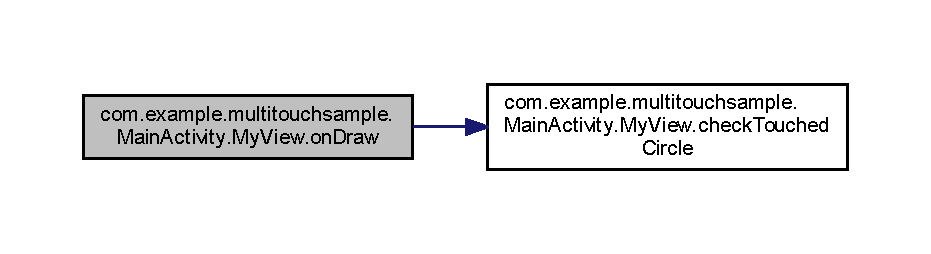
\includegraphics[width=350pt]{classcom_1_1example_1_1multitouchsample_1_1_main_activity_1_1_my_view_a26704cac8a42993a73637404da71988e_cgraph}
\end{center}
\end{figure}


\hypertarget{classcom_1_1example_1_1multitouchsample_1_1_main_activity_1_1_my_view_ab2bf7ce103f9d65b6d677274d51a887e}{}\index{com\+::example\+::multitouchsample\+::\+Main\+Activity\+::\+My\+View@{com\+::example\+::multitouchsample\+::\+Main\+Activity\+::\+My\+View}!on\+Touch\+Event@{on\+Touch\+Event}}
\index{on\+Touch\+Event@{on\+Touch\+Event}!com\+::example\+::multitouchsample\+::\+Main\+Activity\+::\+My\+View@{com\+::example\+::multitouchsample\+::\+Main\+Activity\+::\+My\+View}}
\subsubsection[{on\+Touch\+Event}]{\setlength{\rightskip}{0pt plus 5cm}boolean com.\+example.\+multitouchsample.\+Main\+Activity.\+My\+View.\+on\+Touch\+Event (
\begin{DoxyParamCaption}
\item[{Motion\+Event}]{e}
\end{DoxyParamCaption}
)}\label{classcom_1_1example_1_1multitouchsample_1_1_main_activity_1_1_my_view_ab2bf7ce103f9d65b6d677274d51a887e}


Definition at line 258 of file Main\+Activity.\+java.


\begin{DoxyCode}
259         \{
260             \textcolor{keywordtype}{int} action = e.getAction() & MotionEvent.ACTION\_MASK;
261             
262             \textcolor{keywordflow}{if}(\hyperlink{classcom_1_1example_1_1multitouchsample_1_1_main_activity_1_1_my_view_a45f874e10d05217f17e21ebee2f636ea}{start} == \textcolor{keyword}{false})
263                 \textcolor{keywordflow}{return} \hyperlink{classcom_1_1example_1_1multitouchsample_1_1_main_activity_1_1_my_view_a98da479657a7dabe6b6dee15e39b5a98}{startMultiTouch}(e);
264             \textcolor{keywordflow}{else}
265             \{               
266                 \textcolor{keywordflow}{switch}(action)
267                 \{
268                     \textcolor{keywordflow}{case} MotionEvent.ACTION\_DOWN :
269                     \{
270                         \textcolor{keywordflow}{if}( \hyperlink{classcom_1_1example_1_1multitouchsample_1_1_main_activity_1_1_my_view_a98456bf5be1085790b22ea0179fa2892}{checkTouchedCircle}((\textcolor{keywordtype}{int})e.getX(), (int)e.getY()) == 
      \hyperlink{classcom_1_1example_1_1multitouchsample_1_1_main_activity_1_1_my_view_a90558b5e086112625e29f3941b1444d8}{INVALID\_CIRCLE} )
271                             \textcolor{keywordflow}{return} \textcolor{keyword}{false};
272                         \textcolor{keywordflow}{for}(\textcolor{keywordtype}{int} i=0; i<5; i++)
273                             \hyperlink{classcom_1_1example_1_1multitouchsample_1_1_main_activity_1_1_my_view_a3e8186596771c2fae1397b496be41230}{motion}[i] = -1;
274                         \hyperlink{classcom_1_1example_1_1multitouchsample_1_1_main_activity_1_1_my_view_ab1da26ed65817fe5db4d0be4892ac4b2}{motionStartFlag} = \textcolor{keyword}{true};
275                         Log.d(\textcolor{stringliteral}{"Motion Start"}, \textcolor{stringliteral}{"------------------------------"});
276                     \}
277                     \textcolor{keywordflow}{case} MotionEvent.ACTION\_POINTER\_DOWN :
278                     \{
279                         \textcolor{keywordtype}{int} touchCount = e.getPointerCount();
280                         \textcolor{keywordtype}{int} circleNum = \hyperlink{classcom_1_1example_1_1multitouchsample_1_1_main_activity_1_1_my_view_a98456bf5be1085790b22ea0179fa2892}{checkTouchedCircle}((\textcolor{keywordtype}{int})e.getX(touchCount-1), (
      int)e.getY(touchCount-1));
281                         \textcolor{keywordflow}{if}(touchCount>5 || circleNum == -1 || !\hyperlink{classcom_1_1example_1_1multitouchsample_1_1_main_activity_1_1_my_view_ab1da26ed65817fe5db4d0be4892ac4b2}{motionStartFlag} || !
      \hyperlink{classcom_1_1example_1_1multitouchsample_1_1_main_activity_1_1_my_view_a5df7070a08705a7a8d8aa00a906fa767}{circleAvailable}[circleNum-1])
282                         \{
283                             invalidate();
284                             \textcolor{keywordflow}{return} \textcolor{keyword}{true};
285                         \}
286                                                     
287                         \hyperlink{classcom_1_1example_1_1multitouchsample_1_1_main_activity_1_1_my_view_a5df7070a08705a7a8d8aa00a906fa767}{circleAvailable}[circleNum-1] = \textcolor{keyword}{false};
288                         \hyperlink{classcom_1_1example_1_1multitouchsample_1_1_main_activity_1_1_my_view_a3e8186596771c2fae1397b496be41230}{motion}[circleNum-1] = \hyperlink{classcom_1_1example_1_1multitouchsample_1_1_main_activity_1_1_my_view_ad91938a7ac9667ccd247a072f338a2de}{DIRECTION\_DOT};
289                         
290                         PointF ptf = \textcolor{keyword}{new} PointF();
291                         ptf.x = e.getX(touchCount-1);
292                         ptf.y = e.getY(touchCount-1);
293                         \hyperlink{classcom_1_1example_1_1multitouchsample_1_1_main_activity_1_1_my_view_abf78b5272ae2cffeed639bd024d2a642}{oldPtArr}.add(ptf);
294 
295                         CircleLinkedWithPtId cp = \textcolor{keyword}{new} CircleLinkedWithPtId();
296                         cp.pointerId = e.getPointerId(touchCount-1);
297                         cp.circleNum = circleNum;
298                         \hyperlink{classcom_1_1example_1_1multitouchsample_1_1_main_activity_1_1_my_view_a3bbc2d3fe569814080fe27c6c64eca77}{clp}.add(cp);
299                         
300                         invalidate();
301                         \textcolor{keywordflow}{return} \textcolor{keyword}{true};
302                     \}
303                     
304                     \textcolor{keywordflow}{case} MotionEvent.ACTION\_MOVE :
305                     \{
306                         \hyperlink{classcom_1_1example_1_1multitouchsample_1_1_main_activity_1_1_my_view_ab2213518b7234955478ef54ebdd1db22}{ptArr}.clear();
307                         \hyperlink{classcom_1_1example_1_1multitouchsample_1_1_main_activity_1_1_my_view_a594a2fb9e001c0cfa1aa538c903bc3f8}{plp}.clear();
308                         \textcolor{keywordtype}{int} touchCount = e.getPointerCount();
309                         \textcolor{keywordflow}{if}(touchCount>5)
310                             touchCount = 5;
311                         \textcolor{keywordflow}{for} (\textcolor{keywordtype}{int} i=0; i<touchCount; i++)
312                         \{
313                             PointF ptf = \textcolor{keyword}{new} PointF();
314                             ptf.x = e.getX(i);
315                             ptf.y = e.getY(i);
316                             \hyperlink{classcom_1_1example_1_1multitouchsample_1_1_main_activity_1_1_my_view_ab2213518b7234955478ef54ebdd1db22}{ptArr}.add(ptf);
317                             
318                             PtIdLinkedWithPtIndex pp = \textcolor{keyword}{new} PtIdLinkedWithPtIndex();
319                             pp.pointerIndex = i;
320                             pp.pointerId = e.getPointerId(i);
321                             \hyperlink{classcom_1_1example_1_1multitouchsample_1_1_main_activity_1_1_my_view_a594a2fb9e001c0cfa1aa538c903bc3f8}{plp}.add(pp);
322                             
323                             \hyperlink{classcom_1_1example_1_1multitouchsample_1_1_main_activity_1_1_my_view_a6fbf678025aa07a8024eddeb5431b30c}{checkDirection}(pp, ptf);
324                         \}
325                         invalidate();
326                         \textcolor{keywordflow}{return} \textcolor{keyword}{true};
327                     \}
328                     \textcolor{keywordflow}{case} MotionEvent.ACTION\_POINTER\_UP :
329                     \{
330                         \hyperlink{classcom_1_1example_1_1multitouchsample_1_1_main_activity_1_1_my_view_ab1da26ed65817fe5db4d0be4892ac4b2}{motionStartFlag} = \textcolor{keyword}{false};
331                         
332                         \textcolor{keywordtype}{int} touchCount = e.getPointerCount();
333                         \textcolor{keywordflow}{if}(touchCount>5)
334                             touchCount = 5;
335                         \textcolor{keywordflow}{return} \textcolor{keyword}{true};
336                     \}
337                     \textcolor{keywordflow}{case} MotionEvent.ACTION\_UP :
338                     \{
339                         \textcolor{keywordflow}{if}(!\hyperlink{classcom_1_1example_1_1multitouchsample_1_1_main_activity_1_1_my_view_a10816f1798f68acf937c930b526b112d}{startFlag} && \hyperlink{classcom_1_1example_1_1multitouchsample_1_1_main_activity_1_1_my_view_a45f874e10d05217f17e21ebee2f636ea}{start})
340                         \{
341                             \hyperlink{classcom_1_1example_1_1multitouchsample_1_1_main_activity_1_1_my_view_a10816f1798f68acf937c930b526b112d}{startFlag} = \textcolor{keyword}{true};
342                             \textcolor{keywordflow}{return} \textcolor{keyword}{true};
343                         \}
344                         \textcolor{keywordtype}{int} touchCount = e.getPointerCount();
345                         \textcolor{keywordflow}{if}(touchCount>5)
346                             touchCount = 5;
347                         \hyperlink{classcom_1_1example_1_1multitouchsample_1_1_main_activity_1_1_my_view_aee59904e43e35df3dd7684f22b7dc65d}{motionCheck}();
348                         
349                         \textcolor{comment}{/* initialization for next motion */}
350                         \hyperlink{classcom_1_1example_1_1multitouchsample_1_1_main_activity_1_1_my_view_abf78b5272ae2cffeed639bd024d2a642}{oldPtArr}.clear();
351                         \hyperlink{classcom_1_1example_1_1multitouchsample_1_1_main_activity_1_1_my_view_ab2213518b7234955478ef54ebdd1db22}{ptArr}.clear();
352                         \hyperlink{classcom_1_1example_1_1multitouchsample_1_1_main_activity_1_1_my_view_a3bbc2d3fe569814080fe27c6c64eca77}{clp}.clear();
353                         \hyperlink{classcom_1_1example_1_1multitouchsample_1_1_main_activity_1_1_my_view_a594a2fb9e001c0cfa1aa538c903bc3f8}{plp}.clear();
354                         \textcolor{keywordflow}{for}(\textcolor{keywordtype}{int} i=0; i<5; i++)
355                             \hyperlink{classcom_1_1example_1_1multitouchsample_1_1_main_activity_1_1_my_view_a5df7070a08705a7a8d8aa00a906fa767}{circleAvailable}[i] = \textcolor{keyword}{true};
356                         invalidate();
357                         \textcolor{keywordflow}{return} \textcolor{keyword}{true};
358                     \}
359                     \textcolor{keywordflow}{default} :
360                     \{
361                         invalidate();
362                         \textcolor{keywordflow}{return} \textcolor{keyword}{false};
363                     \}       
364                 \}
365             \}
366         \}
\end{DoxyCode}


Here is the call graph for this function\+:
\nopagebreak
\begin{figure}[H]
\begin{center}
\leavevmode
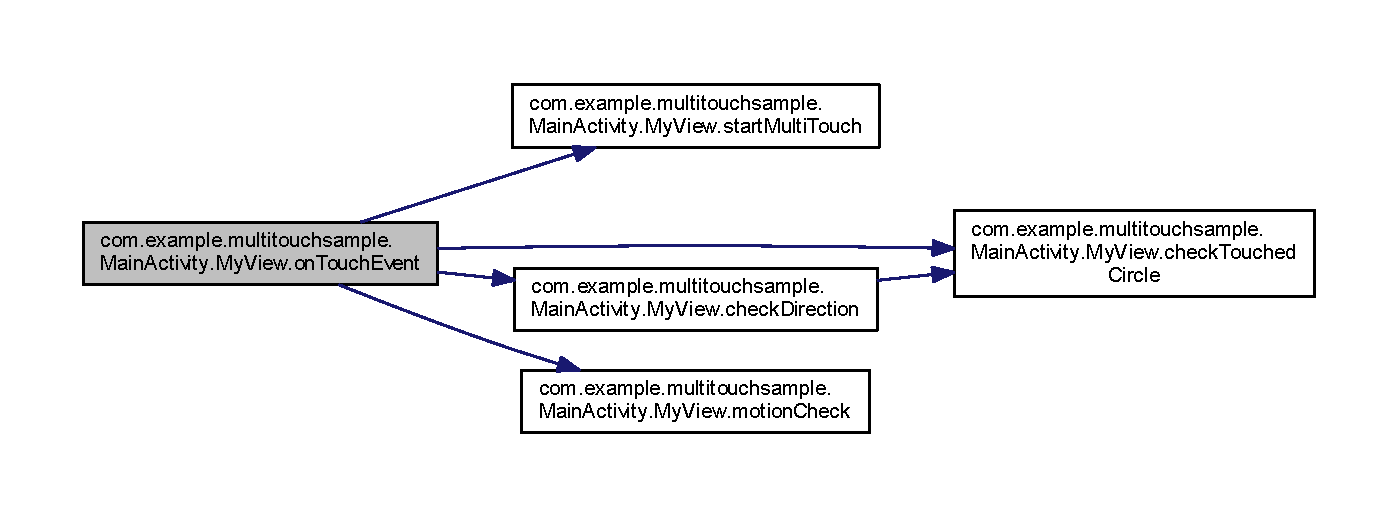
\includegraphics[width=350pt]{classcom_1_1example_1_1multitouchsample_1_1_main_activity_1_1_my_view_ab2bf7ce103f9d65b6d677274d51a887e_cgraph}
\end{center}
\end{figure}


\hypertarget{classcom_1_1example_1_1multitouchsample_1_1_main_activity_1_1_my_view_a98da479657a7dabe6b6dee15e39b5a98}{}\index{com\+::example\+::multitouchsample\+::\+Main\+Activity\+::\+My\+View@{com\+::example\+::multitouchsample\+::\+Main\+Activity\+::\+My\+View}!start\+Multi\+Touch@{start\+Multi\+Touch}}
\index{start\+Multi\+Touch@{start\+Multi\+Touch}!com\+::example\+::multitouchsample\+::\+Main\+Activity\+::\+My\+View@{com\+::example\+::multitouchsample\+::\+Main\+Activity\+::\+My\+View}}
\subsubsection[{start\+Multi\+Touch}]{\setlength{\rightskip}{0pt plus 5cm}com.\+example.\+multitouchsample.\+Main\+Activity.\+My\+View.\+start\+Multi\+Touch (
\begin{DoxyParamCaption}
\item[{Motion\+Event}]{e}
\end{DoxyParamCaption}
)}\label{classcom_1_1example_1_1multitouchsample_1_1_main_activity_1_1_my_view_a98da479657a7dabe6b6dee15e39b5a98}


Function information \+: Start multi touch recognition. 

\begin{DoxyRemark}{Remarks}

\begin{DoxyItemize}
\item Description \+: If \textquotesingle{}num\+Fingers\textquotesingle{} of fingers are touched, set \textquotesingle{}start\textquotesingle{} flag true and start multi touch motion recognition.~\newline
 Set \textquotesingle{}num\+Fingers\textquotesingle{} of starting points. 
\end{DoxyItemize}
\end{DoxyRemark}

\begin{DoxyParams}{Parameters}
{\em e} & A motion event \\
\hline
\end{DoxyParams}
\begin{DoxyReturn}{Returns}
Returns the boolean value of motion event is valid or not.
\end{DoxyReturn}

\begin{DoxyCode}
\textcolor{comment}{// core code}
\end{DoxyCode}
 

Definition at line 463 of file Main\+Activity.\+java.


\begin{DoxyCode}
464         \{
465             \hyperlink{classcom_1_1example_1_1multitouchsample_1_1_main_activity_1_1_my_view_a8e580a64440ed09158aa2bbc50ad4cf6}{startPtArr}.clear();
466             \textcolor{keywordflow}{if} ( e.getAction() == MotionEvent.ACTION\_DOWN || e.getAction() == MotionEvent.ACTION\_MOVE )
467             \{
468                 \textcolor{keywordtype}{int} touchCount = e.getPointerCount();       
469                 \textcolor{keywordflow}{if}(touchCount == 5)
470                 \{
471                     \hyperlink{classcom_1_1example_1_1multitouchsample_1_1_main_activity_1_1_my_view_a45f874e10d05217f17e21ebee2f636ea}{start} = \textcolor{keyword}{true};
472                     Log.d(\textcolor{stringliteral}{"start"} , \textcolor{stringliteral}{"start : "} + \hyperlink{classcom_1_1example_1_1multitouchsample_1_1_main_activity_1_1_my_view_a45f874e10d05217f17e21ebee2f636ea}{start});
473                     \textcolor{keywordflow}{for} (\textcolor{keywordtype}{int} i=0; i<touchCount; i++)
474                     \{
475                         PointF ptf = \textcolor{keyword}{new} PointF();
476                         ptf.x = e.getX(i);
477                         ptf.y = e.getY(i);
478                         \hyperlink{classcom_1_1example_1_1multitouchsample_1_1_main_activity_1_1_my_view_a8e580a64440ed09158aa2bbc50ad4cf6}{startPtArr}.add(ptf);
479                     \}
480                     Collections.sort(\hyperlink{classcom_1_1example_1_1multitouchsample_1_1_main_activity_1_1_my_view_a8e580a64440ed09158aa2bbc50ad4cf6}{startPtArr}, comparatorX);
481                     \textcolor{comment}{/*}
482 \textcolor{comment}{                    PointF pt1, pt2;}
483 \textcolor{comment}{                    pt1 = startPtArr.get(0);}
484 \textcolor{comment}{                    pt2 = startPtArr.get(4);}
485 \textcolor{comment}{                    if(pt2.x-pt1.x < 800)}
486 \textcolor{comment}{                        Collections.sort(startPtArr, comparatorY);}
487 \textcolor{comment}{                    */}
488                     \textcolor{keywordflow}{return} \textcolor{keyword}{true};
489                 \}
490                 \textcolor{keywordflow}{else} \{\textcolor{keywordflow}{return} \textcolor{keyword}{true};\}
491             \}
492             \textcolor{keywordflow}{else} \{\textcolor{keywordflow}{return} \textcolor{keyword}{false};\}
493         \}
\end{DoxyCode}


Here is the caller graph for this function\+:
\nopagebreak
\begin{figure}[H]
\begin{center}
\leavevmode
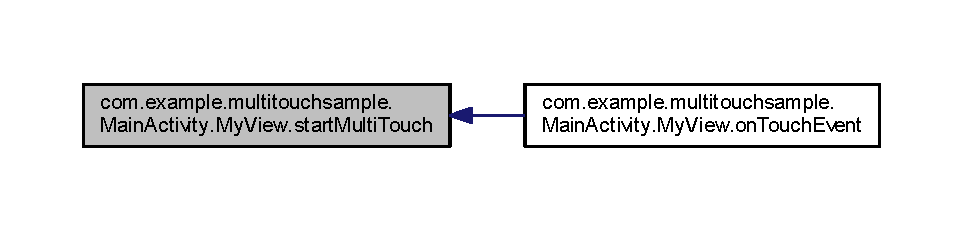
\includegraphics[width=350pt]{classcom_1_1example_1_1multitouchsample_1_1_main_activity_1_1_my_view_a98da479657a7dabe6b6dee15e39b5a98_icgraph}
\end{center}
\end{figure}




\subsection{Member Data Documentation}
\hypertarget{classcom_1_1example_1_1multitouchsample_1_1_main_activity_1_1_my_view_a5df7070a08705a7a8d8aa00a906fa767}{}\index{com\+::example\+::multitouchsample\+::\+Main\+Activity\+::\+My\+View@{com\+::example\+::multitouchsample\+::\+Main\+Activity\+::\+My\+View}!circle\+Available@{circle\+Available}}
\index{circle\+Available@{circle\+Available}!com\+::example\+::multitouchsample\+::\+Main\+Activity\+::\+My\+View@{com\+::example\+::multitouchsample\+::\+Main\+Activity\+::\+My\+View}}
\subsubsection[{circle\+Available}]{\setlength{\rightskip}{0pt plus 5cm}boolean \mbox{[}$\,$\mbox{]} com.\+example.\+multitouchsample.\+Main\+Activity.\+My\+View.\+circle\+Available\hspace{0.3cm}{\ttfamily [private]}}\label{classcom_1_1example_1_1multitouchsample_1_1_main_activity_1_1_my_view_a5df7070a08705a7a8d8aa00a906fa767}


Definition at line 87 of file Main\+Activity.\+java.

\hypertarget{classcom_1_1example_1_1multitouchsample_1_1_main_activity_1_1_my_view_a3bbc2d3fe569814080fe27c6c64eca77}{}\index{com\+::example\+::multitouchsample\+::\+Main\+Activity\+::\+My\+View@{com\+::example\+::multitouchsample\+::\+Main\+Activity\+::\+My\+View}!clp@{clp}}
\index{clp@{clp}!com\+::example\+::multitouchsample\+::\+Main\+Activity\+::\+My\+View@{com\+::example\+::multitouchsample\+::\+Main\+Activity\+::\+My\+View}}
\subsubsection[{clp}]{\setlength{\rightskip}{0pt plus 5cm}Array\+List$<${\bf Circle\+Linked\+With\+Pt\+Id}$>$ com.\+example.\+multitouchsample.\+Main\+Activity.\+My\+View.\+clp\hspace{0.3cm}{\ttfamily [private]}}\label{classcom_1_1example_1_1multitouchsample_1_1_main_activity_1_1_my_view_a3bbc2d3fe569814080fe27c6c64eca77}


Definition at line 100 of file Main\+Activity.\+java.

\hypertarget{classcom_1_1example_1_1multitouchsample_1_1_main_activity_1_1_my_view_ad91938a7ac9667ccd247a072f338a2de}{}\index{com\+::example\+::multitouchsample\+::\+Main\+Activity\+::\+My\+View@{com\+::example\+::multitouchsample\+::\+Main\+Activity\+::\+My\+View}!D\+I\+R\+E\+C\+T\+I\+O\+N\+\_\+\+D\+O\+T@{D\+I\+R\+E\+C\+T\+I\+O\+N\+\_\+\+D\+O\+T}}
\index{D\+I\+R\+E\+C\+T\+I\+O\+N\+\_\+\+D\+O\+T@{D\+I\+R\+E\+C\+T\+I\+O\+N\+\_\+\+D\+O\+T}!com\+::example\+::multitouchsample\+::\+Main\+Activity\+::\+My\+View@{com\+::example\+::multitouchsample\+::\+Main\+Activity\+::\+My\+View}}
\subsubsection[{D\+I\+R\+E\+C\+T\+I\+O\+N\+\_\+\+D\+O\+T}]{\setlength{\rightskip}{0pt plus 5cm}final int com.\+example.\+multitouchsample.\+Main\+Activity.\+My\+View.\+D\+I\+R\+E\+C\+T\+I\+O\+N\+\_\+\+D\+O\+T = 0\hspace{0.3cm}{\ttfamily [static]}, {\ttfamily [private]}}\label{classcom_1_1example_1_1multitouchsample_1_1_main_activity_1_1_my_view_ad91938a7ac9667ccd247a072f338a2de}


Definition at line 92 of file Main\+Activity.\+java.

\hypertarget{classcom_1_1example_1_1multitouchsample_1_1_main_activity_1_1_my_view_afc3ae0a948391b36141f78c515622217}{}\index{com\+::example\+::multitouchsample\+::\+Main\+Activity\+::\+My\+View@{com\+::example\+::multitouchsample\+::\+Main\+Activity\+::\+My\+View}!D\+I\+R\+E\+C\+T\+I\+O\+N\+\_\+\+D\+O\+W\+N@{D\+I\+R\+E\+C\+T\+I\+O\+N\+\_\+\+D\+O\+W\+N}}
\index{D\+I\+R\+E\+C\+T\+I\+O\+N\+\_\+\+D\+O\+W\+N@{D\+I\+R\+E\+C\+T\+I\+O\+N\+\_\+\+D\+O\+W\+N}!com\+::example\+::multitouchsample\+::\+Main\+Activity\+::\+My\+View@{com\+::example\+::multitouchsample\+::\+Main\+Activity\+::\+My\+View}}
\subsubsection[{D\+I\+R\+E\+C\+T\+I\+O\+N\+\_\+\+D\+O\+W\+N}]{\setlength{\rightskip}{0pt plus 5cm}final int com.\+example.\+multitouchsample.\+Main\+Activity.\+My\+View.\+D\+I\+R\+E\+C\+T\+I\+O\+N\+\_\+\+D\+O\+W\+N = 1\hspace{0.3cm}{\ttfamily [static]}, {\ttfamily [private]}}\label{classcom_1_1example_1_1multitouchsample_1_1_main_activity_1_1_my_view_afc3ae0a948391b36141f78c515622217}


Definition at line 93 of file Main\+Activity.\+java.

\hypertarget{classcom_1_1example_1_1multitouchsample_1_1_main_activity_1_1_my_view_aad2a71c46e7cad809a27eb9c4c2600d9}{}\index{com\+::example\+::multitouchsample\+::\+Main\+Activity\+::\+My\+View@{com\+::example\+::multitouchsample\+::\+Main\+Activity\+::\+My\+View}!D\+I\+R\+E\+C\+T\+I\+O\+N\+\_\+\+L\+E\+F\+T@{D\+I\+R\+E\+C\+T\+I\+O\+N\+\_\+\+L\+E\+F\+T}}
\index{D\+I\+R\+E\+C\+T\+I\+O\+N\+\_\+\+L\+E\+F\+T@{D\+I\+R\+E\+C\+T\+I\+O\+N\+\_\+\+L\+E\+F\+T}!com\+::example\+::multitouchsample\+::\+Main\+Activity\+::\+My\+View@{com\+::example\+::multitouchsample\+::\+Main\+Activity\+::\+My\+View}}
\subsubsection[{D\+I\+R\+E\+C\+T\+I\+O\+N\+\_\+\+L\+E\+F\+T}]{\setlength{\rightskip}{0pt plus 5cm}final int com.\+example.\+multitouchsample.\+Main\+Activity.\+My\+View.\+D\+I\+R\+E\+C\+T\+I\+O\+N\+\_\+\+L\+E\+F\+T = 2\hspace{0.3cm}{\ttfamily [static]}, {\ttfamily [private]}}\label{classcom_1_1example_1_1multitouchsample_1_1_main_activity_1_1_my_view_aad2a71c46e7cad809a27eb9c4c2600d9}


Definition at line 94 of file Main\+Activity.\+java.

\hypertarget{classcom_1_1example_1_1multitouchsample_1_1_main_activity_1_1_my_view_a2d1dd293bf4c64feec7de128ef21739e}{}\index{com\+::example\+::multitouchsample\+::\+Main\+Activity\+::\+My\+View@{com\+::example\+::multitouchsample\+::\+Main\+Activity\+::\+My\+View}!D\+I\+R\+E\+C\+T\+I\+O\+N\+\_\+\+R\+I\+G\+H\+T@{D\+I\+R\+E\+C\+T\+I\+O\+N\+\_\+\+R\+I\+G\+H\+T}}
\index{D\+I\+R\+E\+C\+T\+I\+O\+N\+\_\+\+R\+I\+G\+H\+T@{D\+I\+R\+E\+C\+T\+I\+O\+N\+\_\+\+R\+I\+G\+H\+T}!com\+::example\+::multitouchsample\+::\+Main\+Activity\+::\+My\+View@{com\+::example\+::multitouchsample\+::\+Main\+Activity\+::\+My\+View}}
\subsubsection[{D\+I\+R\+E\+C\+T\+I\+O\+N\+\_\+\+R\+I\+G\+H\+T}]{\setlength{\rightskip}{0pt plus 5cm}final int com.\+example.\+multitouchsample.\+Main\+Activity.\+My\+View.\+D\+I\+R\+E\+C\+T\+I\+O\+N\+\_\+\+R\+I\+G\+H\+T = 4\hspace{0.3cm}{\ttfamily [static]}, {\ttfamily [private]}}\label{classcom_1_1example_1_1multitouchsample_1_1_main_activity_1_1_my_view_a2d1dd293bf4c64feec7de128ef21739e}


Definition at line 96 of file Main\+Activity.\+java.

\hypertarget{classcom_1_1example_1_1multitouchsample_1_1_main_activity_1_1_my_view_a43c4159b9b295cfea731211ac614fc0b}{}\index{com\+::example\+::multitouchsample\+::\+Main\+Activity\+::\+My\+View@{com\+::example\+::multitouchsample\+::\+Main\+Activity\+::\+My\+View}!D\+I\+R\+E\+C\+T\+I\+O\+N\+\_\+\+U\+P@{D\+I\+R\+E\+C\+T\+I\+O\+N\+\_\+\+U\+P}}
\index{D\+I\+R\+E\+C\+T\+I\+O\+N\+\_\+\+U\+P@{D\+I\+R\+E\+C\+T\+I\+O\+N\+\_\+\+U\+P}!com\+::example\+::multitouchsample\+::\+Main\+Activity\+::\+My\+View@{com\+::example\+::multitouchsample\+::\+Main\+Activity\+::\+My\+View}}
\subsubsection[{D\+I\+R\+E\+C\+T\+I\+O\+N\+\_\+\+U\+P}]{\setlength{\rightskip}{0pt plus 5cm}final int com.\+example.\+multitouchsample.\+Main\+Activity.\+My\+View.\+D\+I\+R\+E\+C\+T\+I\+O\+N\+\_\+\+U\+P = 3\hspace{0.3cm}{\ttfamily [static]}, {\ttfamily [private]}}\label{classcom_1_1example_1_1multitouchsample_1_1_main_activity_1_1_my_view_a43c4159b9b295cfea731211ac614fc0b}


Definition at line 95 of file Main\+Activity.\+java.

\hypertarget{classcom_1_1example_1_1multitouchsample_1_1_main_activity_1_1_my_view_a90558b5e086112625e29f3941b1444d8}{}\index{com\+::example\+::multitouchsample\+::\+Main\+Activity\+::\+My\+View@{com\+::example\+::multitouchsample\+::\+Main\+Activity\+::\+My\+View}!I\+N\+V\+A\+L\+I\+D\+\_\+\+C\+I\+R\+C\+L\+E@{I\+N\+V\+A\+L\+I\+D\+\_\+\+C\+I\+R\+C\+L\+E}}
\index{I\+N\+V\+A\+L\+I\+D\+\_\+\+C\+I\+R\+C\+L\+E@{I\+N\+V\+A\+L\+I\+D\+\_\+\+C\+I\+R\+C\+L\+E}!com\+::example\+::multitouchsample\+::\+Main\+Activity\+::\+My\+View@{com\+::example\+::multitouchsample\+::\+Main\+Activity\+::\+My\+View}}
\subsubsection[{I\+N\+V\+A\+L\+I\+D\+\_\+\+C\+I\+R\+C\+L\+E}]{\setlength{\rightskip}{0pt plus 5cm}final int com.\+example.\+multitouchsample.\+Main\+Activity.\+My\+View.\+I\+N\+V\+A\+L\+I\+D\+\_\+\+C\+I\+R\+C\+L\+E = -\/1\hspace{0.3cm}{\ttfamily [static]}, {\ttfamily [private]}}\label{classcom_1_1example_1_1multitouchsample_1_1_main_activity_1_1_my_view_a90558b5e086112625e29f3941b1444d8}


Definition at line 90 of file Main\+Activity.\+java.

\hypertarget{classcom_1_1example_1_1multitouchsample_1_1_main_activity_1_1_my_view_a1b17ab3dd378a4846a8de05a58fce3db}{}\index{com\+::example\+::multitouchsample\+::\+Main\+Activity\+::\+My\+View@{com\+::example\+::multitouchsample\+::\+Main\+Activity\+::\+My\+View}!I\+N\+V\+A\+L\+I\+D\+\_\+\+D\+I\+R\+E\+C\+T\+I\+O\+N@{I\+N\+V\+A\+L\+I\+D\+\_\+\+D\+I\+R\+E\+C\+T\+I\+O\+N}}
\index{I\+N\+V\+A\+L\+I\+D\+\_\+\+D\+I\+R\+E\+C\+T\+I\+O\+N@{I\+N\+V\+A\+L\+I\+D\+\_\+\+D\+I\+R\+E\+C\+T\+I\+O\+N}!com\+::example\+::multitouchsample\+::\+Main\+Activity\+::\+My\+View@{com\+::example\+::multitouchsample\+::\+Main\+Activity\+::\+My\+View}}
\subsubsection[{I\+N\+V\+A\+L\+I\+D\+\_\+\+D\+I\+R\+E\+C\+T\+I\+O\+N}]{\setlength{\rightskip}{0pt plus 5cm}final int com.\+example.\+multitouchsample.\+Main\+Activity.\+My\+View.\+I\+N\+V\+A\+L\+I\+D\+\_\+\+D\+I\+R\+E\+C\+T\+I\+O\+N = -\/1\hspace{0.3cm}{\ttfamily [static]}, {\ttfamily [private]}}\label{classcom_1_1example_1_1multitouchsample_1_1_main_activity_1_1_my_view_a1b17ab3dd378a4846a8de05a58fce3db}


Definition at line 91 of file Main\+Activity.\+java.

\hypertarget{classcom_1_1example_1_1multitouchsample_1_1_main_activity_1_1_my_view_a3e8186596771c2fae1397b496be41230}{}\index{com\+::example\+::multitouchsample\+::\+Main\+Activity\+::\+My\+View@{com\+::example\+::multitouchsample\+::\+Main\+Activity\+::\+My\+View}!motion@{motion}}
\index{motion@{motion}!com\+::example\+::multitouchsample\+::\+Main\+Activity\+::\+My\+View@{com\+::example\+::multitouchsample\+::\+Main\+Activity\+::\+My\+View}}
\subsubsection[{motion}]{\setlength{\rightskip}{0pt plus 5cm}int \mbox{[}$\,$\mbox{]} com.\+example.\+multitouchsample.\+Main\+Activity.\+My\+View.\+motion\hspace{0.3cm}{\ttfamily [private]}}\label{classcom_1_1example_1_1multitouchsample_1_1_main_activity_1_1_my_view_a3e8186596771c2fae1397b496be41230}


Definition at line 86 of file Main\+Activity.\+java.

\hypertarget{classcom_1_1example_1_1multitouchsample_1_1_main_activity_1_1_my_view_ab1da26ed65817fe5db4d0be4892ac4b2}{}\index{com\+::example\+::multitouchsample\+::\+Main\+Activity\+::\+My\+View@{com\+::example\+::multitouchsample\+::\+Main\+Activity\+::\+My\+View}!motion\+Start\+Flag@{motion\+Start\+Flag}}
\index{motion\+Start\+Flag@{motion\+Start\+Flag}!com\+::example\+::multitouchsample\+::\+Main\+Activity\+::\+My\+View@{com\+::example\+::multitouchsample\+::\+Main\+Activity\+::\+My\+View}}
\subsubsection[{motion\+Start\+Flag}]{\setlength{\rightskip}{0pt plus 5cm}boolean com.\+example.\+multitouchsample.\+Main\+Activity.\+My\+View.\+motion\+Start\+Flag\hspace{0.3cm}{\ttfamily [private]}}\label{classcom_1_1example_1_1multitouchsample_1_1_main_activity_1_1_my_view_ab1da26ed65817fe5db4d0be4892ac4b2}


Definition at line 88 of file Main\+Activity.\+java.

\hypertarget{classcom_1_1example_1_1multitouchsample_1_1_main_activity_1_1_my_view_abf78b5272ae2cffeed639bd024d2a642}{}\index{com\+::example\+::multitouchsample\+::\+Main\+Activity\+::\+My\+View@{com\+::example\+::multitouchsample\+::\+Main\+Activity\+::\+My\+View}!old\+Pt\+Arr@{old\+Pt\+Arr}}
\index{old\+Pt\+Arr@{old\+Pt\+Arr}!com\+::example\+::multitouchsample\+::\+Main\+Activity\+::\+My\+View@{com\+::example\+::multitouchsample\+::\+Main\+Activity\+::\+My\+View}}
\subsubsection[{old\+Pt\+Arr}]{\setlength{\rightskip}{0pt plus 5cm}Array\+List$<$Point\+F$>$ com.\+example.\+multitouchsample.\+Main\+Activity.\+My\+View.\+old\+Pt\+Arr\hspace{0.3cm}{\ttfamily [private]}}\label{classcom_1_1example_1_1multitouchsample_1_1_main_activity_1_1_my_view_abf78b5272ae2cffeed639bd024d2a642}


Definition at line 103 of file Main\+Activity.\+java.

\hypertarget{classcom_1_1example_1_1multitouchsample_1_1_main_activity_1_1_my_view_a594a2fb9e001c0cfa1aa538c903bc3f8}{}\index{com\+::example\+::multitouchsample\+::\+Main\+Activity\+::\+My\+View@{com\+::example\+::multitouchsample\+::\+Main\+Activity\+::\+My\+View}!plp@{plp}}
\index{plp@{plp}!com\+::example\+::multitouchsample\+::\+Main\+Activity\+::\+My\+View@{com\+::example\+::multitouchsample\+::\+Main\+Activity\+::\+My\+View}}
\subsubsection[{plp}]{\setlength{\rightskip}{0pt plus 5cm}Linked\+List$<${\bf Pt\+Id\+Linked\+With\+Pt\+Index}$>$ com.\+example.\+multitouchsample.\+Main\+Activity.\+My\+View.\+plp\hspace{0.3cm}{\ttfamily [private]}}\label{classcom_1_1example_1_1multitouchsample_1_1_main_activity_1_1_my_view_a594a2fb9e001c0cfa1aa538c903bc3f8}


Definition at line 99 of file Main\+Activity.\+java.

\hypertarget{classcom_1_1example_1_1multitouchsample_1_1_main_activity_1_1_my_view_ab2213518b7234955478ef54ebdd1db22}{}\index{com\+::example\+::multitouchsample\+::\+Main\+Activity\+::\+My\+View@{com\+::example\+::multitouchsample\+::\+Main\+Activity\+::\+My\+View}!pt\+Arr@{pt\+Arr}}
\index{pt\+Arr@{pt\+Arr}!com\+::example\+::multitouchsample\+::\+Main\+Activity\+::\+My\+View@{com\+::example\+::multitouchsample\+::\+Main\+Activity\+::\+My\+View}}
\subsubsection[{pt\+Arr}]{\setlength{\rightskip}{0pt plus 5cm}Array\+List$<$Point\+F$>$ com.\+example.\+multitouchsample.\+Main\+Activity.\+My\+View.\+pt\+Arr\hspace{0.3cm}{\ttfamily [private]}}\label{classcom_1_1example_1_1multitouchsample_1_1_main_activity_1_1_my_view_ab2213518b7234955478ef54ebdd1db22}


Definition at line 104 of file Main\+Activity.\+java.

\hypertarget{classcom_1_1example_1_1multitouchsample_1_1_main_activity_1_1_my_view_a45f874e10d05217f17e21ebee2f636ea}{}\index{com\+::example\+::multitouchsample\+::\+Main\+Activity\+::\+My\+View@{com\+::example\+::multitouchsample\+::\+Main\+Activity\+::\+My\+View}!start@{start}}
\index{start@{start}!com\+::example\+::multitouchsample\+::\+Main\+Activity\+::\+My\+View@{com\+::example\+::multitouchsample\+::\+Main\+Activity\+::\+My\+View}}
\subsubsection[{start}]{\setlength{\rightskip}{0pt plus 5cm}boolean com.\+example.\+multitouchsample.\+Main\+Activity.\+My\+View.\+start\hspace{0.3cm}{\ttfamily [private]}}\label{classcom_1_1example_1_1multitouchsample_1_1_main_activity_1_1_my_view_a45f874e10d05217f17e21ebee2f636ea}


Definition at line 106 of file Main\+Activity.\+java.

\hypertarget{classcom_1_1example_1_1multitouchsample_1_1_main_activity_1_1_my_view_a10816f1798f68acf937c930b526b112d}{}\index{com\+::example\+::multitouchsample\+::\+Main\+Activity\+::\+My\+View@{com\+::example\+::multitouchsample\+::\+Main\+Activity\+::\+My\+View}!start\+Flag@{start\+Flag}}
\index{start\+Flag@{start\+Flag}!com\+::example\+::multitouchsample\+::\+Main\+Activity\+::\+My\+View@{com\+::example\+::multitouchsample\+::\+Main\+Activity\+::\+My\+View}}
\subsubsection[{start\+Flag}]{\setlength{\rightskip}{0pt plus 5cm}boolean com.\+example.\+multitouchsample.\+Main\+Activity.\+My\+View.\+start\+Flag\hspace{0.3cm}{\ttfamily [private]}}\label{classcom_1_1example_1_1multitouchsample_1_1_main_activity_1_1_my_view_a10816f1798f68acf937c930b526b112d}


Definition at line 107 of file Main\+Activity.\+java.

\hypertarget{classcom_1_1example_1_1multitouchsample_1_1_main_activity_1_1_my_view_a8e580a64440ed09158aa2bbc50ad4cf6}{}\index{com\+::example\+::multitouchsample\+::\+Main\+Activity\+::\+My\+View@{com\+::example\+::multitouchsample\+::\+Main\+Activity\+::\+My\+View}!start\+Pt\+Arr@{start\+Pt\+Arr}}
\index{start\+Pt\+Arr@{start\+Pt\+Arr}!com\+::example\+::multitouchsample\+::\+Main\+Activity\+::\+My\+View@{com\+::example\+::multitouchsample\+::\+Main\+Activity\+::\+My\+View}}
\subsubsection[{start\+Pt\+Arr}]{\setlength{\rightskip}{0pt plus 5cm}Array\+List$<$Point\+F$>$ com.\+example.\+multitouchsample.\+Main\+Activity.\+My\+View.\+start\+Pt\+Arr\hspace{0.3cm}{\ttfamily [private]}}\label{classcom_1_1example_1_1multitouchsample_1_1_main_activity_1_1_my_view_a8e580a64440ed09158aa2bbc50ad4cf6}


Definition at line 102 of file Main\+Activity.\+java.

\hypertarget{classcom_1_1example_1_1multitouchsample_1_1_main_activity_1_1_my_view_a677194aa1ca850fc0e716d725f691ba1}{}\index{com\+::example\+::multitouchsample\+::\+Main\+Activity\+::\+My\+View@{com\+::example\+::multitouchsample\+::\+Main\+Activity\+::\+My\+View}!S\+W\+I\+P\+E\+\_\+\+M\+I\+N\+\_\+\+D\+I\+S\+T\+A\+N\+C\+E@{S\+W\+I\+P\+E\+\_\+\+M\+I\+N\+\_\+\+D\+I\+S\+T\+A\+N\+C\+E}}
\index{S\+W\+I\+P\+E\+\_\+\+M\+I\+N\+\_\+\+D\+I\+S\+T\+A\+N\+C\+E@{S\+W\+I\+P\+E\+\_\+\+M\+I\+N\+\_\+\+D\+I\+S\+T\+A\+N\+C\+E}!com\+::example\+::multitouchsample\+::\+Main\+Activity\+::\+My\+View@{com\+::example\+::multitouchsample\+::\+Main\+Activity\+::\+My\+View}}
\subsubsection[{S\+W\+I\+P\+E\+\_\+\+M\+I\+N\+\_\+\+D\+I\+S\+T\+A\+N\+C\+E}]{\setlength{\rightskip}{0pt plus 5cm}final int com.\+example.\+multitouchsample.\+Main\+Activity.\+My\+View.\+S\+W\+I\+P\+E\+\_\+\+M\+I\+N\+\_\+\+D\+I\+S\+T\+A\+N\+C\+E = 140\hspace{0.3cm}{\ttfamily [static]}, {\ttfamily [private]}}\label{classcom_1_1example_1_1multitouchsample_1_1_main_activity_1_1_my_view_a677194aa1ca850fc0e716d725f691ba1}


Definition at line 97 of file Main\+Activity.\+java.



The documentation for this class was generated from the following file\+:\begin{DoxyCompactItemize}
\item 
src/com/example/multitouchsample/\hyperlink{_main_activity_8java}{Main\+Activity.\+java}\end{DoxyCompactItemize}

\hypertarget{classcom_1_1example_1_1multitouchsample_1_1_main_activity_1_1_my_view_1_1_pt_id_linked_with_pt_index}{}\section{com.\+example.\+multitouchsample.\+Main\+Activity.\+My\+View.\+Pt\+Id\+Linked\+With\+Pt\+Index Class Reference}
\label{classcom_1_1example_1_1multitouchsample_1_1_main_activity_1_1_my_view_1_1_pt_id_linked_with_pt_index}\index{com.\+example.\+multitouchsample.\+Main\+Activity.\+My\+View.\+Pt\+Id\+Linked\+With\+Pt\+Index@{com.\+example.\+multitouchsample.\+Main\+Activity.\+My\+View.\+Pt\+Id\+Linked\+With\+Pt\+Index}}


Collaboration diagram for com.\+example.\+multitouchsample.\+Main\+Activity.\+My\+View.\+Pt\+Id\+Linked\+With\+Pt\+Index\+:
\nopagebreak
\begin{figure}[H]
\begin{center}
\leavevmode
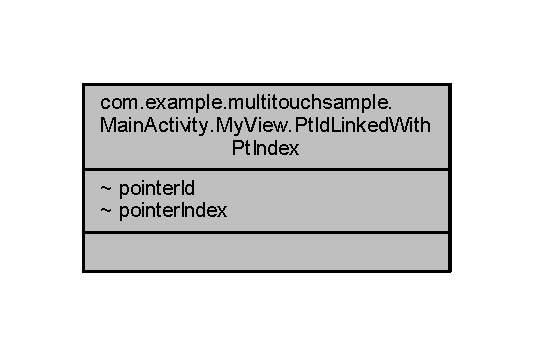
\includegraphics[width=256pt]{classcom_1_1example_1_1multitouchsample_1_1_main_activity_1_1_my_view_1_1_pt_id_linked_with_pt_index__coll__graph}
\end{center}
\end{figure}


\subsection{Detailed Description}
\hyperlink{namespacecom_1_1example_1_1multitouchsample}{com.\+example.\+multitouchsample} ~\newline
 �� \hyperlink{_main_activity_8java}{Main\+Activity.\+java} \hypertarget{classcom_1_1example_1_1multitouchsample_1_1_main_activity_1_1_my_view_1_1_pt_id_linked_with_pt_index_Class}{}\subsection{information}\label{classcom_1_1example_1_1multitouchsample_1_1_main_activity_1_1_my_view_1_1_pt_id_linked_with_pt_index_Class}
\begin{TabularC}{2}
\hline
\rowcolor{lightgray}\PBS\centering {\bf Item }&{\bf Contents  }\\\cline{1-2}
\PBS\centering Company &4\+:00 A.\+M. \\\cline{1-2}
\PBS\centering Author &Park, Hyung Soon \\\cline{1-2}
\PBS\centering Date &2015. 3. 26. \\\cline{1-2}
\end{TabularC}
\hypertarget{classcom_1_1example_1_1multitouchsample_1_1_main_activity_1_1_my_view_1_1_pt_id_linked_with_pt_index_Description}{}\subsection{Description}\label{classcom_1_1example_1_1multitouchsample_1_1_main_activity_1_1_my_view_1_1_pt_id_linked_with_pt_index_Description}

\begin{DoxyItemize}
\item This class will bind pointer\+I\+D with pointer\+Index 
\end{DoxyItemize}

Definition at line 80 of file Main\+Activity.\+java.



The documentation for this class was generated from the following file\+:\begin{DoxyCompactItemize}
\item 
src/com/example/multitouchsample/\hyperlink{_main_activity_8java}{Main\+Activity.\+java}\end{DoxyCompactItemize}

\chapter{File Documentation}
\hypertarget{_main_activity_8java}{}\section{src/com/example/multitouchsample/\+Main\+Activity.java File Reference}
\label{_main_activity_8java}\index{src/com/example/multitouchsample/\+Main\+Activity.\+java@{src/com/example/multitouchsample/\+Main\+Activity.\+java}}
\subsection*{Classes}
\begin{DoxyCompactItemize}
\item 
class \hyperlink{classcom_1_1example_1_1multitouchsample_1_1_main_activity}{com.\+example.\+multitouchsample.\+Main\+Activity}
\item 
class \hyperlink{classcom_1_1example_1_1multitouchsample_1_1_main_activity_1_1_my_view}{com.\+example.\+multitouchsample.\+Main\+Activity.\+My\+View}
\item 
class \hyperlink{classcom_1_1example_1_1multitouchsample_1_1_main_activity_1_1_my_view_1_1_circle_linked_with_pt_id}{com.\+example.\+multitouchsample.\+Main\+Activity.\+My\+View.\+Circle\+Linked\+With\+Pt\+Id}
\item 
class \hyperlink{classcom_1_1example_1_1multitouchsample_1_1_main_activity_1_1_my_view_1_1_pt_id_linked_with_pt_index}{com.\+example.\+multitouchsample.\+Main\+Activity.\+My\+View.\+Pt\+Id\+Linked\+With\+Pt\+Index}
\end{DoxyCompactItemize}
\subsection*{Packages}
\begin{DoxyCompactItemize}
\item 
package \hyperlink{namespacecom_1_1example_1_1multitouchsample}{com.\+example.\+multitouchsample}
\end{DoxyCompactItemize}

%--- End generated contents ---

% Index
\backmatter
\newpage
\phantomsection
\clearemptydoublepage
\addcontentsline{toc}{chapter}{Index}
\printindex

\end{document}
